%%%%%%%%%%%%%%%%%%%%%%%%%%%%%%%%%%%%%%%%%
% Masters/Doctoral Thesis 
% LaTeX Template
% Version 2.5 (27/8/17)
%
% This template was downloaded from:
% http://www.LaTeXTemplates.com
%
% Version 2.x major modifications by:
% Vel (vel@latextemplates.com)
%
% This template is based on a template by:
% Steve Gunn (http://users.ecs.soton.ac.uk/srg/softwaretools/document/templates/)
% Sunil Patel (http://www.sunilpatel.co.uk/thesis-template/)
%
% Template license:
% CC BY-NC-SA 3.0 (http://creativecommons.org/licenses/by-nc-sa/3.0/)
%
%%%%%%%%%%%%%%%%%%%%%%%%%%%%%%%%%%%%%%%%%

%----------------------------------------------------------------------------------------
%	PACKAGES AND OTHER DOCUMENT CONFIGURATIONS
%----------------------------------------------------------------------------------------

\documentclass[
11pt, % The default document font size, options: 10pt, 11pt, 12pt
%oneside, % Two side (alternating margins) for binding byhttps://v1.overleaf.com/20740335gynbkgcvnmvs# default, uncomment to switch to one side
english, % ngerman for German
singlespacing, % Single line spacing, alternatives: onehalfspacing or doublespacing
%draft, % Uncomment to enable draft mode (no pictures, no links, overfull hboxes indicated)
%nolistspacing, % If the document is onehalfspacing or doublespacing, uncomment this to set spacing in lists to single
%liststotoc, % Uncomment to add the list of figures/tables/etc to the table of contents
%toctotoc, % Uncomment to add the main table of contents to the table of contents
%parskip, % Uncomment to add space between paragraphs
%nohyperref, % Uncomment to not load the hyperref package
headsepline, % Uncomment to get a line under the header
%chapterinoneline, % Uncomment to place the chapter title next to the number on one line
%consistentlayout, % Uncomment to change the layout of the declaration, abstract and acknowledgements pages to match the default layout
]{MastersDoctoralThesis} % The class file specifying the document structure

\usepackage[utf8]{inputenc} % Required for inputting international characters
\usepackage[T1]{fontenc} % Output font encoding for international characters

\usepackage{mathpazo} % Use the Palatino font by default
%\usepackage[backend=bibtex,style=authoryear,natbib=true]{biblatex} % Use the bibtex backend with the authoryear citation style (which resembles APA)
\usepackage[backend=bibtex]{biblatex} % Use the bibtex backend with the 
%authoryear citation style (which resembles APA)

\addbibresource{Thesis.bib} % The filename of the bibliography

%\usepackage[autostyle=true]{csquotes} % Required to generate 
%%language-dependent quotes in the bibliography


\usepackage{graphicx}
\usepackage{wrapfig}
\usepackage{pdflscape}
\usepackage{mathtools}


\usepackage{amsthm}

\newcommand{\projectName}{CROSSMINER~}
\newcommand{\CROSSMINER}{CROSSMINER~}
\newcommand{\projectNameNoT}{CROSSMINER}

\newcommand{\cc}[1]{\multicolumn{1}{c}{#1}}
\newcolumntype{d}[1]{D{.}{.}{#1}}
\newcommand{\code}[1]{{\texttt{#1}}}
\newcommand{\codefoot}[1]{{\texttt{#1}}}

\newcommand{\CrossSim}{\textsc{CrossSim}\xspace}
\newcommand{\CrossSimA}{\textsc{CrossSim}}

\newcommand{\MUDABlue}{\textsc{MUDABlue}\xspace}
\newcommand{\CLAN}{\textsc{CLAN}\xspace}
\newcommand{\RepoPal}{\textsc{RepoPal}\xspace}

\usepackage{xspace}
\newcommand*{\ie}{i.e.,\@\xspace}
\newcommand*{\eg}{e.g.,\@\xspace}
\newcommand*{\cf}{cf.\@\xspace}






%----------------------------------------------------------------------------------------
%	MARGIN SETTINGS
%----------------------------------------------------------------------------------------

\geometry{
	paper=a4paper, % Change to letterpaper for US letter
	inner=2.5cm, % Inner margin
	outer=3.8cm, % Outer margin
	bindingoffset=.5cm, % Binding offset
	top=1.5cm, % Top margin
	bottom=1.5cm, % Bottom margin
	%showframe, % Uncomment to show how the type block is set on the page
}

%----------------------------------------------------------------------------------------
%	THESIS INFORMATION
%----------------------------------------------------------------------------------------

\thesistitle{Automated Approaches \\to Assess the Similarity of Open Source Software Projects} % Your thesis title, this is used in the title and abstract, print it elsewhere with \ttitle
%title and abstract, print it elsewhere with \ttitle
%\supervisor{Prof. Dr. Davide \textsc{Di Ruscio} \\ Dr. Phuong T. Nguyen} % Your supervisor's name, this is used in the title page, print it elsewhere with \supname
\supervisor{Dr. Davide \textsc{Di Ruscio}}
\examiner{abc} % Your examiner's name, this is not currently used anywhere in the template, print it elsewhere with \examname
\degree{Master of Science} % Your degree name, this is used in the title page and abstract, print it elsewhere with \degreename
\author{Riccardo \textsc{Rubei}} % Your name, this is used in the title page and abstract, print it elsewhere with \authorname
\addresses{} % Your address, this is not currently used anywhere in the template, print it elsewhere with \addressname

\subject{Computer Science} % Your subject area, this is not currently used anywhere in the template, print it elsewhere with \subjectname
\keywords{} % Keywords for your thesis, this is not currently used anywhere in the template, print it elsewhere with \keywordnames
\university{\href{http://www.univaq.it}{University of L'Aquila}} % Your 
%university's name and URL, this is used in the title page and abstract, print 
%it elsewhere with \univname
\department{\href{http://www.disim.univaq.it/}{Department of Information 
Engineering Computer Science and Mathematics}} % Your department's name and 
%URL, this is used in the title page and abstract, print it elsewhere with 
%\deptname
\group{\href{http://researchgroup.university.com}{The Software Architecture Group}} % Your research group's name and URL, this is used in the title page, print it elsewhere with \groupname
\faculty{\href{http://faculty.university.com}{Faculty Name}} % Your faculty's name and URL, this is used in the title page and abstract, print it elsewhere with \facname

\AtBeginDocument{
\hypersetup{pdftitle=\ttitle} % Set the PDF's title to your title
\hypersetup{pdfauthor=\authorname} % Set the PDF's author to your name
\hypersetup{pdfkeywords=\keywordnames} % Set the PDF's keywords to your keywords
}

\begin{document}

\frontmatter % Use roman page numbering style (i, ii, iii, iv...) for the pre-content pages

\pagestyle{plain} % Default to the plain heading style until the thesis style is called for the body content

%----------------------------------------------------------------------------------------
%	TITLE PAGE
%----------------------------------------------------------------------------------------




	\begin{titlepage}
		\begin{center}
			
			\vspace*{.06\textheight}
			
			
\includegraphics[width=0.2\linewidth]{images/univaq}
			
			{\scshape\LARGE \univname\par}\vspace{1.5cm} % University name
			\textsc{\Large Master Thesis}\\[0.5cm] % Thesis type
			
			\HRule \\[0.4cm] % Horizontal line
			{\huge \bfseries \ttitle\par}\vspace{0.4cm} % Thesis title
			\HRule \\[1.5cm] % Horizontal line
			
			\begin{minipage}[t]{0.4\textwidth}
				\begin{flushleft} \large
					\emph{Author:}\\
					\href{http://www.johnsmith.com}{\authorname} % Author name - remove the \href bracket to remove the link
				\end{flushleft}
			\end{minipage}
			\begin{minipage}[t]{0.4\textwidth}
				\begin{flushright} \large
					\emph{Supervisor:} \\
					\href{http://www.di.univaq.it/diruscio/index.php}{\supname} \\% Supervisor name - remove the 
					%\href 
					%bracket to remove the link  
					\emph{Co-supervisor:}\\
					\href{https://github.com/phuongthanhnguyen}{Dr. Phuong T. Nguyen} % Supervisor name - remove 
					%the 
					%\href 
				\end{flushright}
			\end{minipage}\\[2.5cm]
			
			\vfill
			
			\large \textit{Corso di Laurea Magistrale in Informatica}\\[0.3cm] % 
			%University 
			%requirement text
			\textit{}\\[0.4cm]
			%\groupname\\
			\deptname\\[2cm] % Research group name and department name
			
			\vfill
			
			{\large Academic Year 2017/2018}\\[4cm] % Date
			%
\includegraphics{Logo} % University/department logo - uncomment to place it
			
			\vfill
		\end{center}
	\end{titlepage}

%----------------------------------------------------------------------------------------
%	DECLARATION PAGE
%----------------------------------------------------------------------------------------








%\begin{declaration}
%\addchaptertocentry{\authorshipname} % Add the declaration to the table of contents
%\noindent I, \authorname, declare that this thesis titled, \enquote{\ttitle} and the work presented in it are my own. I confirm that:
%
%\begin{itemize} 
%\item This work was done wholly or mainly while in candidature for a research degree at this University.
%\item Where any part of this thesis has previously been submitted for a degree or any other qualification at this University or any other institution, this has been clearly stated.
%\item Where I have consulted the published work of others, this is always clearly attributed.
%\item Where I have quoted from the work of others, the source is always given. With the exception of such quotations, this thesis is entirely my own work.
%\item I have acknowledged all main sources of help.
%\item Where the thesis is based on work done by myself jointly with others, I have made clear exactly what was done by others and what I have contributed myself.\\
%\end{itemize}
% 
%\noindent Signed:\\
%\rule[0.5em]{25em}{0.5pt} % This prints a line for the signature
% 
%\noindent Date:\\
%\rule[0.5em]{25em}{0.5pt} % This prints a line to write the date
%\end{declaration}




%\cleardoublepage

%----------------------------------------------------------------------------------------
%	QUOTATION PAGE
%----------------------------------------------------------------------------------------

\vspace*{0.2\textheight}

%\noindent\enquote{\itshape Thanks to my solid academic training, today I can write hundreds of words on virtually any topic without possessing a shred of information, which is how I got a good job in journalism.}\bigbreak
%\hfill Dave Barry

%----------------------------------------------------------------------------------------
%	ABSTRACT PAGE
%----------------------------------------------------------------------------------------

%\begin{abstract}
%\addchaptertocentry{\abstractname} % Add the abstract to the table of contents
%The Thesis Abstract is written here (and usually kept to just this page). The page is kept centered vertically so can expand into the blank space above the title too\ldots
%\end{abstract}

%----------------------------------------------------------------------------------------
%	ACKNOWLEDGEMENTS
%----------------------------------------------------------------------------------------

\begin{acknowledgements}
\addchaptertocentry{\acknowledgementname} % Add the acknowledgements to the table of contents %The acknowledgments and the people to thank go here, don't forget to include your project advisor\ldots

I would like to express my deepest and sincerest gratitude to my supervisor, Prof. Dr. Davide Di Ruscio, for his expert guidance, constructive criticism, continuous support and encouragement throughout my study. It has been a privilege to work with him and I hope to have the chance to continue working under his supervision in the future.

I would also like to thank my co-supervisor Dr. Phuong T. Nguyen for his supports, as well as for his patience, since he has been always available for comments and suggestions.

A special thank to Dr. Juri Di Rocco for his help, in particular during the implementation phase of the software tools. His great expertise has been always a good source of inspiration for me. %helped me a lot.

Also a big thank goes to my dear friends Roberta, Andrea, Claudio, Francesco, Riccardo, Cristina, Rodolfo, who sustained me during my master degree and who never let me go mad.

Finally I would like to thank my mother and my family, without them I could not have been able to complete my study.

\end{acknowledgements}

%----------------------------------------------------------------------------------------
%	LIST OF CONTENTS/FIGURES/TABLES PAGES
%----------------------------------------------------------------------------------------

\tableofcontents % Prints the main table of contents

\listoffigures % Prints the list of figures

\listoftables % Prints the list of tables

%----------------------------------------------------------------------------------------
%	ABBREVIATIONS
%----------------------------------------------------------------------------------------

%\begin{abbreviations}{ll} % Include a list of abbreviations (a table of two columns)
%
%\textbf{LAH} & \textbf{L}ist \textbf{A}bbreviations \textbf{H}ere\\
%\textbf{WSF} & \textbf{W}hat (it) \textbf{S}tands \textbf{F}or\\
%
%\end{abbreviations}



%----------------------------------------------------------------------------------------
%	PHYSICAL CONSTANTS/OTHER DEFINITIONS
%----------------------------------------------------------------------------------------

%\begin{constants}{lr@{${}={}$}l} % The list of physical constants is a three column table
%
%% The \SI{}{} command is provided by the siunitx package, see its documentation for instructions on how to use it
%
%Speed of Light & $c_{0}$ & \SI{2.99792458e8}{\meter\per\second} (exact)\\
%%Constant Name & $Symbol$ & $Constant Value$ with units\\
%
%\end{constants}


%----------------------------------------------------------------------------------------
%	SYMBOLS
%----------------------------------------------------------------------------------------

%\begin{symbols}{lll} % Include a list of Symbols (a three column table)
%
%$a$ & distance & \si{\meter} \\
%$P$ & power & \si{\watt} (\si{\joule\per\second}) \\
%%Symbol & Name & Unit \\
%
%\addlinespace % Gap to separate the Roman symbols from the Greek
%
%$\omega$ & angular frequency & \si{\radian} \\
%
%\end{symbols}

%----------------------------------------------------------------------------------------
%	DEDICATION
%----------------------------------------------------------------------------------------

%\dedicatory{For/Dedicated to/To my\ldots} 

%----------------------------------------------------------------------------------------
%	THESIS CONTENT - CHAPTERS
%----------------------------------------------------------------------------------------




\mainmatter % Begin numeric (1,2,3...) page numbering

\pagestyle{thesis} % Return the page headers back to the "thesis" style

% Include the chapters of the thesis as separate files from the Chapters folder
% Uncomment the lines as you write the chapters








	
	
	\chapter{Introduction}
	\label{sec:Introduction}
	\subsection{Summary}
Open source software (OSS) repositories contain a large amount of data that has been accumulated along the software development process. Not only source code but also metadata available from different related sources, e.g. communication channels, bug tracking systems, is beneficial to the development process once it is properly mined. Research has been performed to understand and predict software evolution, exploiting the rich metadata available at OSS repositories. This allows for the reduction of effort in knowledge acquisition and quality gain. Developers can leverage the underlying knowledge if they are equipped with suitable tools. For instance, it is possible to empower IDEs by means of tools that continuously monitor the developer's activities and contexts in order to activate dedicated recommendation engines \cite{Ponzanelli:2014:MST:2597073.2597077}. 

%To aim for software quality, for developers it is necessary to understand how similar, mature projects are developed.   it is necessary

To aim for software quality, developers normally build their project by learning from mature OSS projects having comparable functionalities. To this end, the ability to search for similar software projects with respect to different criteria such as functionalities and dependencies plays an important role in the development process. Two projects are deemed to be similar if they implement some features being described by the same abstraction, even though they may contain various functionalities for different domains \cite{McMillan:2012:DSS:2337223.2337267}. Understanding the similarities between open source software projects allows for reusing of source code and prototyping, or choosing alternative implementations \cite{Schafer:2007:CFR:1768197.1768208},\cite{10.1109/SANER.2017.7884605}, thereby improving software quality. Meanwhile measuring the similarities between developers and software projects is a critical phase for most types of recommender systems \cite{DBLP:conf/rweb/NoiaO15},\cite{Sarwar:2001:ICF:371920.372071}. Similarities are used as a base by both content-based and collaborative-filtering recommender systems to choose the most suitable and meaningful items for a given item \cite{Schafer:2007:CFR:1768197.1768208}. Failing to compute precise similarities means concurrently adding a decline in the overall performance of these systems. Nevertheless, measuring similarities between software systems has been considered as a daunting task \cite{Chen:2015:SFD:2684822.2685305},\cite{McMillan:2012:DSS:2337223.2337267}. Furthermore, considering the miscellaneousness of artifacts in open source software repositories, similarity computation becomes more complicated as many artifacts and several cross relationships prevail.

In recent years, considerable effort has been made to provide automated assistance to developers in navigating large information spaces and giving recommendations. Though remarkable progress can be seen in this field, there is still room for improvement. To the best of our knowledge, most of the existing approaches consider the constituent components of the OSS ecosystem separately, without paying much attention to their mutual connections. There is a lack of a proper scheme that facilitates a unified consideration of various OSS artifacts and recommendations. 

CROSSMINER\footnote{\url{https://www.crossminer.org}} is a research project funded by the EU Horizon 2020 Research and Innovation Programme, aiming at supporting the development of complex software systems by \textit{i)} enabling monitoring, in-depth analysis and evidence-based selection of open source components, and \textit{ii)} facilitating knowledge extraction from large OSS repositories \cite{10.1007/978-3-319-74730-9_33}. In the context of the project, we work towards an advanced Eclipse-based IDE providing intelligent recommendations that go far beyond the current \emph{code completion-oriented} practice. Among others, an indispensable functionality is to find a set of similar OSS projects to a given project with respect to different criteria, such as external dependencies, application domain, or API usage \cite{NDRDSEAA2018},\cite{DBLP:conf/iir/NDD013}.

The purpose of this thesis is the implementation of two approaches, MUDABlue and Clan, with the aim of compare the results of new tool by CROSSMINER development team (CrossSim). CROSSSIM (Cross Project Relationships for Computing Open Source Software Similarity), is an approach that makes use of graphs for rep-resenting different kinds of relationships in the OSS ecosystem. In particular, with the adoption of the graph representation, we are able to transform the relationships among non-human artifacts, e.g. API utilizations, source code, interactions, and humans, e.g. developers into a mathematically computable format, i.e. one that
facilitates various types of computation techniques. Naturally this kind of approaches has to be evaluated, and confronted with others similar tools. My work helps addressing this challenge providing these two tools and evaluating all the results to show how nice is CrossSim.
	\clearpage
	
	%	\section{The CROSSMINER Project}
	%	\label{sec:CROSSMINER}
	%	\input{src/CROSSMINER}
	%	\clearpage
	
	\chapter{Mathematical Background}
	\label{sec:MathsBackground}
	



%\section{Overview}

In the field of Information Retrieval \cite{Manning:2008:IIR:1394399}, there are techniques being widely used in several applications. They can be considered as a basic and indispensable part of a knowledge mining system. Throughout this deliverable some techniques are utilized in different similarity computation algorithms and thus it is worth conducting a review of them. Among others, Term-Document Matrix, Cosine Similarity, Latent Semantic Analysis and Jaccard Index are going to be briefly recalled due to their popularity. Furthermore, later in the chapter we also provide a brief introduction to a graph algorithm \cite{Jeh:2002:SMS:775047.775126}, which has been exploited to compute the similarity among OSS projects \cite{NDRDSEAA2018}.

%This section presents an overview of existing approaches that have been devised over the last decade to detect similar software systems. To this end a mathematical background, which is common to knowledge mining systems, is discussed in Sec. \ref{sec:mathBackground}. %Section \ref{sec:overview} presents an overview of existing software similarity measurement techniques.

%The and they serve as a base for further presentation.

%%%%%%%%%%%%%%%%%%%%%%%%%%%%%%%%%%%%%%%%%%%%%%%%%%%%%%%%%%

%\section{String-Based}

%Text similarity measures play an increasingly important role in text related research and applications in tasks such as information retrieval, text classification, document clustering, topic detection, topic tracking, questions generation, question answering, essay scoring, short answer scoring, machine translation, text summarization and others. Finding similarity between words is a fundamental part of text similarity which is then used as a primary stage for sentence, paragraph and document similarities. There two way in which words can be similar each other, lexically if they share sequences of characters similar and  semantically if are used in the same context, used in the same way and so on. 

%The world of lexical similarity con be divided in two categories: character-based and word-based. To better understand what character-based means, here one of the most well known technique: Levenshtein distance.

%\section{Levenshtein distance}
% Levenshtein distance defines distance between two strings by counting the minimum number of operations needed to transform one string into the other, where an operation is defined as an insertion, deletion, or substitution of a single character, or a transposition of two adjacent characters.
%
%This is an example:
%
%\begin{itemize}
%    \item kitten to sitten (substitution of "s" for "k").
%    \item sitten to sittin (substitution of "i" for "e").
%    \item sittin to sitting (insertion of "g" at the end).
%\end{itemize}
%
%Moving to the word-based,  the word or string similarity measures operate on string sequences and character composition. A string metric is a metric that measures similarity or dissimilarity (distance) between two text strings for approximate string matching or comparison.




\section{Term-Document Matrix} \label{sec:TDM}
In Natural Language Processing \cite{Collobert:2011:NLP:1953048.2078186}, a term-document matrix (TDM) is used to represent the relationships between words and documents \cite{Turney:2010:FMV:1861751.1861756}. In a TDM, each row corresponds to a document and each column corresponds to a term. A cell in the TDM represents the weight of a term in a document. The most common weighting scheme used in document retrieval is the \emph{term frequency-inverse document frequency (tf-idf)} function \cite{Reed:2006:TNT:1193211.1193734}. If we consider a set of $n$ documents $D=(d_{1},d_{2},..,d_{n})$ and a set of terms $t=(t_{1},t_{2},..,t_{r})$ then the representation of a document $d \in D $ is vector $\vec{\delta}=(w_{1}^{d},w_{2}^{d},..,w_{r}^{d})$, where the weight $w_{k}^{d}$ of term $k$ in document $d$ is computed using the {\em tf-idf} function \cite{Ramos1999}:

\begin{equation} \label{tfidf} %\nonumber 
w_{k}^{d} =tf\cdot idf(k,d,D)= f_{k}^{d}\cdot log\frac{n}{\left | \left \{ d\in D: t_{k} \in d \right \} \right |} 
\end{equation}

where $f_{k}^{d}$ is the frequency of term $t_{k}$ in document $d$.

Another common weighting scheme uses only the frequency of terms in documents for cells in TDM, \ie the number of occurrence of a term in a document, instead of {\em tf-idf}. As an example, we consider a set of two simple documents $D=(doc_{a},doc_{b})$ as given below:

\begin{itemize}
	\item[+] \textbf{doc}$_a$: \emph{Julie loves me more than Linda loves me.}
	\item[+] \textbf{doc}$_b$: \emph{Jane likes me more than Julie loves me.}
\end{itemize}

\begin{wrapfigure}{!h}{0.5\textwidth}
	\centering
	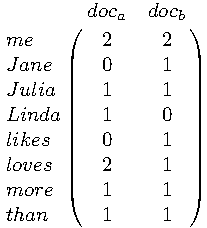
\includegraphics[width=0.25\textwidth]{images/TDMExample.pdf}
	\caption{An example of a Term-Document Matrix}
	\label{fig:TDMExample}
\end{wrapfigure}

The corresponding term-document matrix for $D$ is depicted in Figure \ref{fig:TDMExample}.

%The set of terms $t$ consists of $6$ elements, i.e. $t=(she$, $is$, $today$, $a$, $nice$, $city)$ and 

TDM has been exploited to characterize software systems and finally to compute similarities between them \cite{10.1109/APSEC.2004.69},\cite{10.1109ICPC.2016.7503721},\cite{McMillan:2012:DSS:2337223.2337267}. In a TDM for software systems, each row represents a package, an API call or a function and each column represents a software system. A cell in the matrix is the number of occurrence of a package/an API/function in each corresponding software system. A TDM for software systems has a similar form to the matrix shown in Figure~\ref{fig:TDMExample} where documents are replaced by software systems and terms are replaced by API calls.


\section{Cosine Similarity} \label{sec:CosineSimilarity}

Cosine similarity is a metric used to compute similarity between two objects using their feature vectors \cite{tversky1977features}. An object is characterized as a vector, and for a pair of vectors $\vec{\alpha}=(\alpha_{1},\alpha_{2},..,\alpha_{n})$ and $\vec{\beta}=(\beta_{1},\beta_{2},..,\beta_{n})$ there is an angle between them. Intuitively, the cosine similarity metric measures the similarity as the cosine of the corresponding angle between the two vectors and it is computed using the inner product as follows. 

\begin{equation} \label{eqn:Cosine}
CosineSim(\vec{\alpha},\vec{\beta}) = \frac{\sum_{i=1}^{n}\alpha_{i}\cdot \beta_{i}}{\sqrt{\sum_{i=1}^{n}(\alpha_{i})^{2} }\cdot \sqrt{\sum_{i=1}^{n}(\beta_{i})^{2}}}
\end{equation}

Figure \ref{fig:Cosine} illustrates the cosine similarity between two vectors $\vec{\alpha}$ and $\vec{\beta}$ in a three-dimension space. This can be thought as the similarity between two documents with three terms $t=(t_{1},t_{2},t_{3})$.

\begin{figure}[h!]
	\centering
	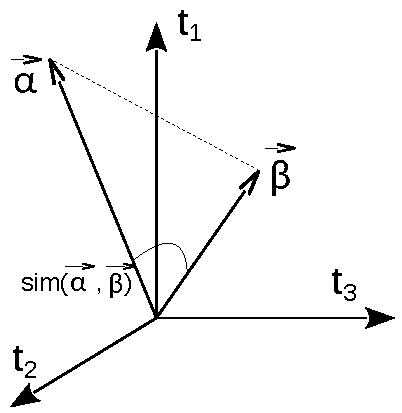
\includegraphics[width=0.25\textwidth]{images/Cosine.pdf}
	\caption{Cosine similarity between two feature vectors $\vec{\alpha}$ and $\vec{\beta}$}
	\label{fig:Cosine}
\end{figure}

Refer to the example in Section~\ref{sec:TDM}, the two documents are represented by means of two vectors as follows: 

%From the strings is possible to count the occurrencies of each term, putting everything in a matrix.
%Since in this kind of evaluation is not important the meaning or where the words are, is possibile to create the related vectore in order to compute the similarity.\\
%This is an example of how the cosine similarity can be done  between two sentences. These are the two string that we want to compare to see how much they are related each other.
%
	\begin{equation} \nonumber
	\vec{doc_a} = [2, 0, 1, 1, 0, 2, 1, 1]
	\end{equation}
	\begin{equation} \nonumber
	\vec{doc_b} = [2, 1, 1, 0, 1, 1, 1, 1]
	\end{equation}

And the similarity between them is computed using Equation~\ref{eqn:Cosine}: 

\begin{equation} %\label{eqn:Cosine}
CosineSim(\vec{doc_a},\vec{doc_b}) = \frac{9}{\sqrt{12}\cdot \sqrt{10}} = 0.822
\end{equation}

A similarity score of $0.822$ implies that these documents are highly similar.% each other 0.822, in a range between 0.0 and 1.0.

Cosine similarity has been popularly adopted in many applications that are related to similarity measurement in various domains \cite{Huang:2012:LCD:2343876.2343884},\cite{Islam:2008:STS:1376815.1376819},\cite{Linden:2003:ARI:642462.642471},\cite{conf:iscis:MadylovaO09},\cite{Mihalcea:2006:CKM:1597538.1597662}. Among the similarity metrics being recalled in this deliverable, the prevalence of Cosine Similarity is obvious as it is utilized in almost all of them as follows: \textit{MUDABlue} \cite{10.1109/APSEC.2004.69}, \textit{CLAN} \cite{McMillan:2012:DSS:2337223.2337267}, \textit{CLANdroid} \cite{10.1109ICPC.2016.7503721}, \textit{LibRec} \cite{6671293}, \textit{SimApp} \cite{Chen:2015:SFD:2684822.2685305}, \textit{WuKong} \cite{Wang:2015:WSA:2771783.2771795}, \textit{TagSim} \cite{Lo:2012:DSA:2473496.2473616}, and \textit{RepoPal} \cite{10.1109/SANER.2017.7884605}.


%%%%%%%%%%%%%%%%%%%%%%%%%%%%%%%%%%%%%%%%%%%%%%%%%%%%%%%%%  
%\section{Corpus-Based}




\section{Latent Semantic Analysis}

The problem with the term-document matrix is that the intrinsic relationships among different terms of a document cannot fully be captured. Furthermore, same words can be used to explain different requirements or the other way around, the same requirements can be described using different words \cite{10.1109/APSEC.2004.69}. Latent Semantic Analysis (LSA), also known as Latent Semantic Indexing (LSI), has been proposed to overcome these problems \cite{Landauer1998}. The technique exploits a mathematical model that can infer latent semantic relationships to compute similarity. LSA represents the contextual usage meaning of words by statistical computations applied to a large corpus of text. It then generates a representation that captures the similarity of words and text passages. To perform LSA on a text, a term-document matrix is created to characterize the text. Afterwards, Singular Value Decomposition (SVD) - a matrix decomposition technique - is used in combination with LSA to reduce matrix dimensionality \cite{kb2005}. SVD takes a highly variable set of data entries as input and transforms to a lower dimensional space but reveals the substructure of the original data. Essentially, it decomposes a rectangular matrix into the product of three other matrices as given in Equation ~\ref{eqn:Decomposition} \cite{kb2005}. Correspondingly, the decomposition is depicted in Figure~\ref{fig:Decomposition}.

\begin{equation} \label{eqn:Decomposition}
A_{mn}=U_{mm}S_{mn}V_{mn}^{T}
\end{equation}

in which

\begin{itemize}
	\item $U_{mm}$: Orthogonal matrix.
	\item $S_{mn}$: Diagonal matrix.
	\item $V_{mn}^{T}$: The transpose of an orthogonal matrix.
%	\item $X$: Low Rank matrix.
\end{itemize}


Figure~\ref{fig:Decomposition} depicts the low rank reduction phase. The new matrix is the product of the other three, but reducted, this is a very relevant issue. If the singular values in $S_{mn}$ are ordered by size, the first $k$ largest may be kept and the remaining smaller ones set to zero. The product of the resulting matrices is a matrix $X$ which is only approximately equal to $A_{mm}$ , and is of rank $k$. It can be shown that the new matrix $X$ is the matrix of rank $k$ which is closest in the least squares sense to $A_{mm}$. The amount of dimension reduction, i.e., the choice of $k$, is critical to our work. Ideally, we want a value of k that is large enough to fit all the real structure in the data, but small enough so that we do not also fit the sampling error or unimportant details. The proper way to make such choices is an open issue in the factor analytic literature. In practice, we currently use an operational criterion - a value of $k$ which yields good retrieval performance.%\\ In our work we decided a \emph{k value =} $\frac{repository}{2}$

\begin{figure}[h!]
	\centering
	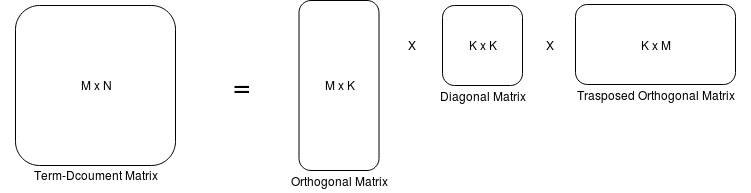
\includegraphics[width=15cm,height=20cm,keepaspectratio]{images/LSIk.png}
	\caption{The decomposition phase}
	\label{fig:Decomposition}
\end{figure}


$U_{mm}$ describes the original row entities as vectors of derived orthogonal factor values. $S_{mn}$ represents the original column entities in the same way, and $V_{mn}$ is a diagonal matrix containing scaling values. With the application of LSA it is possible to find the most relevant features and remove the least important ones by means of the reduced matrix $U_{mm}$. As a result, an equivalence of $A_{mm}$ can be constructed using the most relevant features. LSA helps reveal the latent relationship among words as well as among passages which cannot be guaranteed by a simple term-document matrix. The similarity measurement by LSA reflects adequately human perception of similarity and association among texts. Using LSA, similarities among documents are measured as the cosine of the angle between their row vectors (see Section~\ref{sec:CosineSimilarity}). LSA has been applied in \cite{10.1109/APSEC.2004.69},\cite{10.1109ICPC.2016.7503721},\cite{McMillan:2012:DSS:2337223.2337267} to compute similarities of software systems. The main disadvantage of LSA is that it is computational expensive when a large amount of information is analyzed.

%\newpage
%An example.

To illustrate how LSA works, we take an example with a set of $9$ documents as follows: %Image that these are a set of document to be analyzed and we want to apply the procedure stated before.

\begin{itemize}
	\item \textbf{doc}$_1$: \emph{Human machine interface for ABC computer applications.}
	\item \textbf{doc}$_2$: \emph{A survey of user opinion of computer system response time.}
	\item \textbf{doc}$_3$: \emph{The EPS user interface management system.}
	\item \textbf{doc}$_4$: \emph{System and human system engineering testing of EPS.}
	\item \textbf{doc}$_5$: \emph{Relation of user perceived response time to error measurement.}
	\item \textbf{doc}$_6$: \emph{The generation of random, binary, ordered trees.}
	\item \textbf{doc}$_7$: \emph{The intersection graph of paths in trees.}
	\item \textbf{doc}$_8$: \emph{Graph minors IV: Widths of trees and well-quasi-ordering.}
	\item \textbf{doc}$_9$: \emph{Graph minors: A survey.}
\end{itemize}

The term-document matrix for the document set is shown in Figure~\ref{fig:TermDocumentMatrix}.

\begin{figure}[h!]
	\centering
	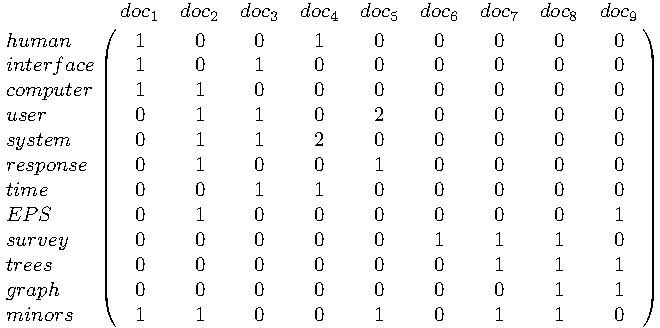
\includegraphics[width=0.8\textwidth]{images/TermDocumentMatrix.pdf}
	\caption{Term-Document Matrix of the example}
	\label{fig:TermDocumentMatrix}
\end{figure}

A computation exploiting an LSA implementation yields the matrices in Figures~\ref{fig:UmmMatrix},~\ref{fig:SmnMatrix}, and~\ref{fig:VmnMatrix}.Let's consider the \cite{Landauer1998} example to better explain how does the LSA works.

\begin{figure}[h!]
	\centering
	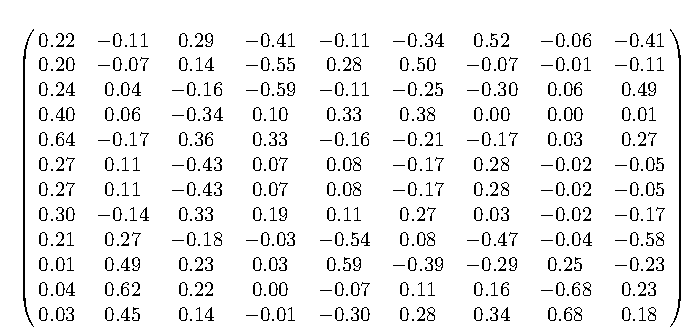
\includegraphics[width=0.8\textwidth]{images/UmmMatrix.pdf}
	\caption{Matrix $U_{mm}$x}
	\label{fig:UmmMatrix}
\end{figure}


\begin{figure}[h!]
	\centering
	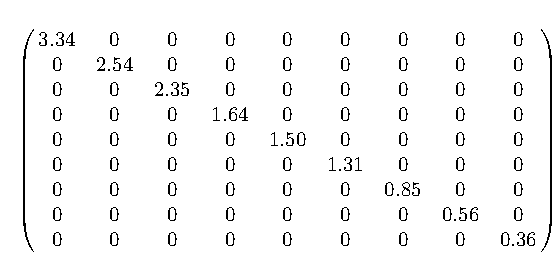
\includegraphics[width=0.68\textwidth]{images/SmnMatrix.pdf}
		\caption{Matrix $S_{mn}$}
	\label{fig:SmnMatrix}
\end{figure}


\begin{figure}[h!]
	\centering
	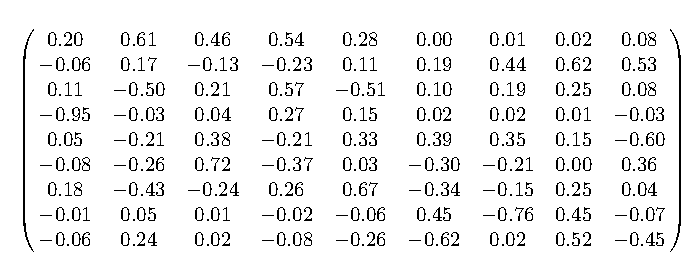
\includegraphics[width=0.8\textwidth]{images/VmnMatrix.pdf}
	\caption{Matrix $S_{mn}$}
	\label{fig:VmnMatrix}
\end{figure}

Figure~\ref{fig:DecomposedMatrix} depict the result of the decomposition with a rank of 2.

\begin{figure}[h!]
	\centering
	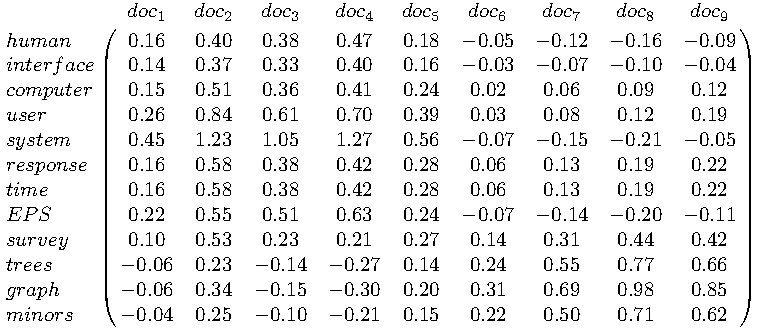
\includegraphics[width=0.9\textwidth]{images/DecomposedMatrix.pdf}
	\caption{The recovered matrix}
	\label{fig:DecomposedMatrix}
\end{figure}






\section{Jaccard Index}\label{sec:jaccard}

Given two objects $\alpha$ and $\beta$ represented by their corresponding set of elements $O(\alpha)$ and $O(\beta)$, the similarity is computed as the ratio of the cardinality of the intersection and the cardinality of the union of the two sets. The formula is given below:

\begin{equation} \label{eqn:Jaccard}
Jaccard(\alpha,\beta)=\frac{|O(\alpha)\bigcap O(\beta)|}{|O(\alpha)\bigcup O(\beta)|} 
\end{equation}

\begin{figure}[h!]
	\centering
	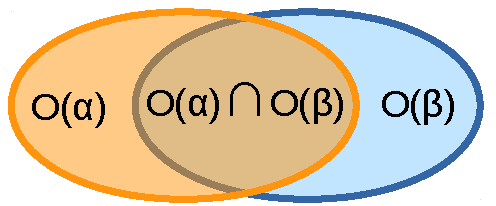
\includegraphics[width=0.4\textwidth]{images/JaccardSimilarity.pdf}
	\caption{Jaccard similarity between two sets $O(\alpha)$ and $O(\beta)$}
	\label{fig:Jaccard}
\end{figure}

The similarity using the Jaccard index is visualized in Figure \ref{fig:Jaccard}. The eclipse on the left hand represents $O(\alpha)$ and the eclipse on the right hand represents $O(\beta)$. The intersection of the two sets is $O(\alpha)\bigcap O(\beta)$ and the larger it is, the closer to $1$ is the Jaccard index. Once the two sets completely overlap each other, $Jaccard(\alpha,\beta)$ is equal to $1$. Among the similarity tools presented in this thesis, \textit{AnDarwin} \cite{Crussell2013} and \textit{RepoPal} \cite{10.1109/SANER.2017.7884605} employ Jaccard index in their implementation. %Furthermore, as a baseline for our evaluation, the index is used to compute similarity between two projects using their sets of dependencies (Section \ref{sec:CrossSimEvaluation}).



\section{Graph Similarity} \label{sec:GraphSimilarity}
Graph similarity is an active research field and receives a significant attention from the research community. In this section, we are going to review the approaches for computing similarity in graph that are beneficial to our context. A directed graph is defined as a tuple $G=(V,E,R)$, where $V$ is the set of vertices, $E$ is the set of edges and $R$ represents the relationship among the nodes. A graph consists of enormous nodes and oriented links with semantic relationships. A triple <$subject, predicate, object$> with $subject, object \in V$ and $predicate \in E$ states that node $subject$ is connected to node $object$ by means of the edge labelled with $predicate$. To evaluate the similarity of two nodes in a graph, their intrinsic characteristics like nodes, links, and their mutual interactions are incorporated into the similarity calculation \cite{DiNoia:2012:LOD:2362499.2362501},\cite{Nguyen:2015:CRV:2942298.2942305},\cite{Nguyen:2015:ESP:2740908.2742141}. Among others, feature-based semantic similarity metrics gauge the similarity between graph nodes as a measure of commonality and distinction of their hallmarks.

Tversky provides a deep insight into feature-based similarity in his work \cite{tversky1977features}. There, objects are represented as a set of common and distinctive features and the similarity between two objects is computed by comparing their features. An object is represented in one of the following forms: \emph{binary values}, \emph{nominal values}, \emph{ordinal values}, and \emph{cardinal values}. Feature-based semantic similarity metrics first attempt to characterize resources in a graph as sets of feature and then perform similarity calculation on them.

%Measuring similarity using features is based on the premise that the more common features two objects hold, the more similar they are. 
%Bearing on this principle, f
%the similarity between 

%In the following sub-sections, we are going to review three algorithms for computing similarity in graphs. These algorithms serve as base for our proposed approach that exploits the graph structure to compute similarity.

%\subsection{SimRank} \label{sec:SimRank}

\begin{figure}[h!]
	\centering
	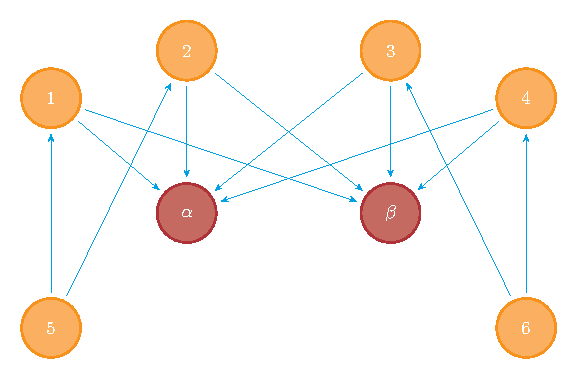
\includegraphics[width=0.60\textwidth]{images/SimRank.pdf}
	\caption{SimRank similarity}
	\label{fig:SimRank}
\end{figure}

SimRank has been designed to calculate similarity based on the mutual relationships between nodes \cite{Jeh:2002:SMS:775047.775126}. In a graph, the similarity between two nodes is dependent on their neighbors. Considering two nodes, the more similar nodes point to them, the more similar the two nodes are. For example, in Figure \ref{fig:SimRank}, the two nodes $\alpha$ and $\beta $ are highly similar because they are concurrently pointed by other four nodes in the graph. Also, node $1$ is similar to node $2$ since both are pointed by node $5$. Comparably, the similarity between node $3$ and node $4$ is high as they are pointed by node $6$. In this sense, the similarity between two nodes $\alpha$ and $\beta$ is computed by using a fixed-point function. Given $k \geq 0$ we have $R^{(k)}(\alpha,\beta) = 1$ with $\alpha = \beta$ and $R^{(k)}(\alpha,\beta) = 0$ with $k=0$ and $\alpha \neq \beta$. In all the other cases the general formula is:

\begin{equation}\label{eqn:SimRank}
R^{(k+1)}(\alpha,\beta) = 
\frac{\Delta}{|I(\alpha)|\cdot|I(\beta)|}\sum_{i=1}^{|I(\alpha)|}\sum_{j=1}^{|I(\beta)|}R^{(k)}(I_{i}(\alpha),I_{j}(\beta))
\end{equation}

where $\Delta$ is a damping factor ($0 \leq \Delta < 1$); $I(\alpha)$ and $I(\beta)$ are the set of incoming neighbors of $\alpha$ and $\beta$, respectively. $|I(\alpha)|\cdot|I(\beta)|$ is the factor used to normalize the sum, thus making $R^{(k)}(\alpha,\beta) \in [0,1]$. Equation~\ref{eqn:SimRank} implies that the similarity for two nodes is computed by aggregating the similarity of all possible pairs of their neighbors. 

SimRank has been used by \CrossSim  \cite{NDRDSEAA2018} as the mechanism to compute the similarity among nodes in a graph representing the OSS ecosystem.






%\clearpage
%%%%%%%%%%%%%%%%%%%%%%%%%%%%%%%%%%%%%%%%%%%%%%%%%%%%%%%%%%  
%\section{Knowledge-Based}
%Knowledge-Based Similarity aims to identify the degree of similarity between words using informations derived from semantic networks.
%Knowledge-based similarity measures can be divided roughly into two groups: measures of semantic similarity and measures of semantic relatedness.By semantic similarity we mean concepts that are related each other on the basis of their likeness.
%Semantic relatedness, on the other hand, is a more general notion of relatedness, not specifically tied to the shape or form of the concept. Semantic similarity is a metric defined over a set of documents or terms, where the idea of distance between them is based on the likeness of their meaning or semantic content as opposed to similarity which can be estimated regarding their syntactical representation (e.g. their string format).
%An example of relatedness is the Lask algorithm which identify senses of words in context using definition overlap. To clarify let's take a look an example in \cite{Resnik}.
%Using the Oxford Advanced Learner's Dictionary, it finds that word \emph{pine} has two senses:
%\begin{itemize}
%	\item{Sense 1: kind of \textbf{evergreen tree} with needle-shaped leaves}
%	\item{Sense 2: waste away through sorrow ir illness.}
%\end{itemize}
%
%The word \emph{cone} has three senses:
%\begin{itemize}
%	\item{Sense 1: solid body which narrows to a point}
%	\item{Sense 2: something of this shape whether solid or hollow}
%	\item{Sense 3: fruit of certain \textbf{evergreen tree}}
%\end{itemize}
%
%Each of the two senses of the word \emph{pine} is compared with each of the three senses of the \emph{cone} and it is found that the words \emph{evergreen tree} occurs in one sense each of the two words. These two senses are then declared to be the most appropriate senses when words \emph{pine} and \emph{cone} are used togheter.
%
%Concerning the similarity an example could be Resnik(1995) which uses the information content of concepts, computed from their frequency of occurrence in a large corpus, to determine the semantic relatedness of word senses\cite{Resnik}.
%Another example is Jian \& Conrath \cite{Jian}s It combines a lexical taxonomy structure with corpus statistical information so that the semantic distance between nodes in the semantic space constructed by the taxonomy can be better quantified with the computational evidence derived from a distributional analysis of corpus data. Specifically, the proposed measure is a combined approach that inherits the edge-based approach of the edge counting scheme, which is then enhanced by the node-based approach of the information content calculation.


	\clearpage
	
	
	\chapter{Literature Review on Software Similarity Measurement}	
	\label{sec:LiteratureReview}
	%=============================================================================================================================================================================================
%: (\emph{i}) Low-level Similarity: Computing similarity between app using low-level data, e.g: source code, byte code, function calls, API reference, etc. (\emph{ii}) High-level Similarity: Detecting the semantic similarity using metadata, such as: topic distribution, readme file, description, star events, etc.%This classification is used throughout this paper as a means to distinguish between the approaches with regards to the input information used for similarity computation.
%A pre-processing stage is performed to extract identifiers such as variable names, function names and to remove unrelated factors such as comment. With the application of Latent Semantic Analysis, software is considered as a document and each identifier is considered as a word. LSA is used for extracting and representing the contextual usage meaning of words by statistical computations applied to a large corpus of text. 
%$CLAN$ works based on the document framework for computing similarity, semantic anchors, e.g. those that define the documents' semantic features. Semantic anchors and dependencies help obtain a more precise value for similarity computation between documents. The assumption is that if two applications have API calls implementing requirements described by the same abstraction, then the two applications are more similar than those that do not have common API calls. The approach uses API calls as semantic anchors to compute application similarity since API calls contain precisely defined semantics. The similarity between applications is computed by matching the semantics already expressed in the API calls.
%However, $CLAN$ is claimed to help obtain a higher precision than that of $MUDABlue$. 
%\paragraph{Low-level Similarity}  Together with a tool for automatically categorizing open source repositories, t
%, which have been conceived to measure the similarity between different software systems
%makes an overview of existing approaches. 
%Each technique has been conceived to address specific issues as summarized below. In the next sections, we make an overview of existing approaches dealing with the problem of detecting similar software systems.
%=============================================================================================================================================================================================





The ability to search for similar software projects with respect to different criteria such as functionalities and dependencies plays an important role in the development process. Two projects are deemed to be similar if they implement some features being described by the same abstraction, even though they may contain various functionalities for different domains \cite{McMillan:2012:DSS:2337223.2337267}. Understanding the similarities between open source software projects allows for reusing of source code and prototyping, or choosing alternative implementations \cite{Schafer:2007:CFR:1768197.1768208},\cite{10.1109/SANER.2017.7884605}, thereby improving software quality. Meanwhile measuring the similarities between developers and software projects is a critical phase for most types of recommender systems \cite{DBLP:conf/rweb/NoiaO15},\cite{Sarwar:2001:ICF:371920.372071}. Similarities are used as a base by both content-based and collaborative-filtering recommender systems to choose the most suitable and meaningful items for a given item \cite{Schafer:2007:CFR:1768197.1768208}. Failing to compute precise similarities means concurrently adding a decline in the overall performance of these systems. Nevertheless, measuring similarities between software systems has been considered as a daunting task \cite{Chen:2015:SFD:2684822.2685305},\cite{McMillan:2012:DSS:2337223.2337267}. Furthermore, considering the miscellaneousness of artifacts in open source software repositories, similarity computation becomes more complicated as many artifacts and several cross relationships prevail. Choosing the right tool to compute similarity is. This thesis is dedicated to the problem of software similarity computation. In particular, we present our work related to.

In recent years, several approaches have been proposed to solve the problem of software similarity computation. In this chapter, we review some of the most notable approaches which have been conceived to measure the similarity between software systems or OSS projects. Afterwards, in Section~\ref{sec:Analysis} we analyze their characteristics. According to \cite{Chen:2015:SFD:2684822.2685305}, depending on the set of mined features, there are two main types of software similarity computation techniques: 

\begin{itemize}	
	\item \textit{Low-level Similarity}: it is calculated by considering low-level data, e.g., source code, byte code, function calls, API reference, etc.; 
	\item \textit{High-level Similarity}: detecting the semantic similarity using metadata, such as: topic distribution, readme file, description, star events, etc. Source code is not taken into account.	
\end{itemize}

This classification is used throughout this paper as a means to distinguish between the approaches with regards to the input information used for similarity computation. In particular, we review the following categories of software similarity:

\begin{itemize}
	\item Detecting similar open source applications (see Sections~\ref{sec:mudablue},~\ref{sec:clan},~\ref{sec:tagsim}, and~\ref{sec:repopal}).
	\item Detecting similar mobile applications (see Sections~\ref{sec:clandroid},~\ref{sec:SimApp}, and~\ref{sec:andarwin}).
	\item Detecting software plagiarisms and clones (see Sections~\ref{sec:gplag} and~\ref{sec:wukong}).
	\item Recommending reusable libraries (see Section~\ref{sec:librec}).
\end{itemize}


%\section{Computing software similarities} \label{sec:SimilarityMeasurement}


%=============================================================================================================================================================================================
%%%%\textit{\textbf{Low-level similarity}.} It is calculated by considering low-level data, e.g., source code, byte code, function calls, API reference, etc. The authors in \cite{10.1109/APSEC.2004.69} propose  MUDABlue, an approach for computing similarity between software projects using source code. To compute similarities between software systems, MUDABlue first extracts identifiers from source code and removes unrelated content. It then creates an identifier-software matrix where each row corresponds to one identifier and each column corresponds to a software system. Afterwards, it removes too rare or too popular identifiers. Finally, latent semantic analysis (LSA) \cite{landauer2006latent} is performed on the identifier-software matrix to compute similarity on the reduced matrix using cosine similarity. CLAN (Closely reLated ApplicatioNs) \cite{McMillan:2012:DSS:2337223.2337267} is an approach for automatically detecting similar Java applications by exploiting the semantic layers corresponding to packages class hierarchies.  CLAN represents source code files as a term document matrix (TDM), in which a row contains a unique class or package and a column corresponds to an application. Singular value decomposition is then applied to reduce the matrix dimensionality. Similarity between applications is computed as the cosine similarity between vectors in the reduced matrix. 

%MUDABlue and CLAN are comparably similar in the way they represent software and identifiers/API in a term-document matrix and then apply LSA to compute similarities. CLAN includes API calls for computing similarity, whereas MUDABlue integrates every word in source code files into the term-document matrix. As a result, the similarity scores of CLAN reflect better the perception of humans of similarity than those of MUDABlue \cite{McMillan:2012:DSS:2337223.2337267}. %This makes the difference in the performance of the two algorithms

%Inspired by $CLAN$, $CLANdroid$ was developed for detecting similar Android applications with the assumption that similar apps share some semantic anchors \cite{10.1109ICPC.2016.7503721}. By extending the scope of semantic anchors for Android apps, starting from APK (Android Package) $CLANdroid$ extracts features, i.e. identifiers, intents from source code, API calls and sensors from JAR files and user permissions from \emph{AndroidManifest.xml}\footnote{\href{https://developer.android.com/guide/topics/manifest/manifest-intro.html}{Android App Manifest}}. For each feature, a feature-Application Matrix is built, resulting in five different matrices. Latent Semantic Indexing is applied to all the matrices to reduce the dimensionality. Afterwards, similarity between a pair of applications is computed as the cosine similarity between their corresponding feature vectors from the matrix. Users can query for similar apps with a given app by specifying which feature is taken into consideration. 
%\paragraph{High-level Similarity}
%The framework is built using a combination of rule mining and collaborative filtering techniques. It finds a set of relevant libraries, based on the current set of libraries that a project already uses. Association rule mining is applied to find similar libraries that co-exist in many projects. 
%$LibRec$ suggests the inclusion of libraries that may be useful for a given project. 
%By $SimApp$, if two apps implement related semantic requirements then they are seen as similar. 
%Through the use of a set of training data, the optimal weights are determined by means of online learning techniques. 
%Tags are terms that are used to highlight the most important characteristics of software systems and therefore, they help users narrow down the search scope. 
%Rather than other approaches that exploit low-level implementation, 

%%%\textit{\textbf{High-level similarity}.} It is calculated by considering project metadata, such as topic distribution, README files, textual descriptions, star events (if available e.g., in GitHub), etc. In \cite{6671293} authors propose LibRec, a library recommendation technique to help developers leverage existing libraries. LibRec employs association rule mining and collaborative filtering techniques to search for top most similar projects and recommends libraries used by these projects to a given project. A project is characterized by a feature vector where each entry corresponds to the occurrence of a library and the similarity between two projects is computed as the similarity between their feature vectors. 

%SimApp has been proposed to find mobile applications with similar semantic requirements \cite{Chen:2015:SFD:2684822.2685305}. The metric makes use of high-level metadata collected from application stores for detecting similar mobile applications. Each mobile application is modeled by a set of features, so called \emph{modalities}. For each of the features, a kernel function is derived to calculate the similarity between applications. The final similarity score for a pair of applications is a linear combination of the multiple kernels with weights. 
%In \cite{Lo:2012:DSA:2473496.2473616} tags are leveraged to characterize applications and then to compute similarity between them. The proposed approach can be used to detect similar applications written in different languages. Based on the hypothesis that tags capture better the intrinsic features of applications compared to textual descriptions, the approach extracts tags attached to an application and computes their weights \cite{Lo:2012:DSA:2473496.2473616}. This information forms the features of a given software system and is used to distinguish it from others. An application is characterized by a feature vector with each entry corresponding to the weight of a tag. Eventually, the similarity between two applications is computed using cosine similarity.
%=============================================================================================================================================================================================



\section{MUDABlue: Automatic Categorization for Open Source Repositories}\label{sec:mudablue}


Together with a tool for automatically categorizing open source repositories, the authors in \cite{10.1109/APSEC.2004.69} propose an approach for computing similarity between software projects using source code. A pre-processing stage is performed to extract identifiers such as variable names, function names and to remove unrelated factors such as comment.

With the application of Latent Semantic Analysis, software is considered as a document and each identifier is considered as a word. LSA is used for extracting and representing the contextual usage meaning of words by statistical computations applied to a large corpus of text. In summary, MUDABlue works in the following steps to compute similarities between software systems:

\begin{itemize}
	
	\item[i)] Extracts identifiers from source code and removes unrelated content;
	\item[ii)] Creates an identifier-software matrix with each row corresponds to one identifier and each column corresponds to a software system;%by considering software system as a document and an identifier as a word;
	\item[iii)] Removes unimportant identifiers, i.e. those that are too rare or too popular;
	\item[iv)] Performs LSA on the identifier-software matrix and computes similarity on the reduced matrix using cosine similarity; 
\end{itemize}

MUDABlue has been evaluated on a database consisting of software systems written in C \cite{10.1109/APSEC.2004.69}. The outcomes of the evaluation were compared against two existing approaches, namely GURU \cite{Maarek:1991:IRA:126244.126254}, and the SVM based method by \emph{Ugurel et al} \cite{Ugurel:2002:WCA:775047.775141}. The evaluation shows that MUDABlue outperforms these observed algorithms with regards to precision and recall.


\section{CLAN: Finding Related Applications}\label{sec:clan}

CLAN (Closely reLated ApplicatioNs) \cite{McMillan:2012:DSS:2337223.2337267} is an approach for automatically detecting similar Java applications by exploiting the semantic layers corresponding to packages class hierarchies. CLAN works based on the document framework for computing similarity, semantic anchors, e.g. those that define the documents' semantic features. Semantic anchors and dependencies help obtain a more precise value for similarity computation between documents. The assumption is that if two applications have API calls implementing requirements described by the same abstraction, then the two applications are more similar than those that do not have common API calls. The approach uses API calls as semantic anchors to compute application similarity since API calls contain precisely defined semantics. The similarity between applications is computed by matching the semantics already expressed in the API calls.

Using a complete software application as input, CLAN represents source code files as a TDM, in which a row contains a unique class or package and a column corresponds to an application. SVD is then applied to reduce the dimension of the matrix. Similarity between applications is computed as the cosine similarity between vector in the reduced matrix. CLAN has been tested on a dataset with more than $8.000$ SourceForge\footnote{SourceForge: \url{https://sourceforge.net/}} applications and shows that it qualifies for the detection of similar applications \cite{McMillan:2012:DSS:2337223.2337267}.

MUDABlue and CLAN are comparable in the way they represent software and source code components like variables, function names or API calls in a term-document matrix and then apply LSA to find the similarity and to category the softwares. However, CLAN has been claimed to help obtain a higher precision than that of MUDABlue as it considers only API calls to represent software systems. 


\section{TagSim: Collaborative Tagging to Detect Similar Applications}\label{sec:tagsim}

In \cite{Lo:2012:DSA:2473496.2473616} tags are leveraged to characterize applications and then to compute similarity between them. Tags are terms that are used to highlight the most important characteristics of software systems \cite{xia:tag:2013} and therefore, they help users narrow down the search scope. Some examples of tags are the category of an app, the license of the system, the programming languages. TagSim\footnote{For the sake of clarity, in this thesis we give a name for the algorithms that have not been named originally} can be used to detect similar applications written in different languages. Based on the assumption that tags capture better the intrinsic features of applications compared to textual descriptions, TagSim extracts tags attached to an application and computes their weights. This information forms the features of a given software system and can be used to distinguish it from others. The technique also differentiates between important tags and unimportant based on their frequency of appearance in the analyzed software systems. The more popular a tag across the applications is, the less important it is and vice versa, i.e. the weight of tag $t$ is $w(t) = \frac{1}{|App(t)|}$ where $App(t)$ is the set of applications that have $t$ as tag. Each application is characterized by a feature vector, $\vec{Tag(a)}$, with each entry corresponds to the weight of a tag the application has. Eventually, the similarity between two applications is computed as the cosine similarity between the two vectors:

\begin{equation}
sim(a_{1},a_{2})= CosineSim(\vec{Tag(a_{1})},\vec{Tag(a_{2})})
%\frac{\sum_{t\in Tag(a_{1})\bigcap Tag(a_{2})}w_{t,a_{1}}\times w_{t,a_{2}}}{\sqrt{\sum_{t\in Tag(a_{1})}(w_{t,a_{1}})^{2} }\times \sqrt{\sum_{t\in Tag(a_{2})}(w_{t,a_{2}})^{2}}} 
\end{equation}

To evaluate TagSim, the authors in \cite{Lo:2012:DSA:2473496.2473616} collected and analyzed more than a hundred thousands of projects. A total of $20$ queries were used to study the performance of the algorithm in comparison with CLAN. The authors also performed a user study to manually analyze the extent to which two applications are similar. Afterwards, success rate, confidence, and precision were used as evaluation metrics. The experimental results show that TagSim helps achieve better performance in comparison to CLAN with a success rate of $80\%$.

Similarly, to help users category a new software object, $TagCombine$ has been proposed in \cite{xia:tag:2013}. $TagCombine$ works using three components: a multi-label ranking component, a similarity based ranking component, and a tag-term based ranking component. In this approach, tags are also used to represent a piece of software as a feature vector, and finally to compute similarity. $TagCombine$ has been evaluated against the approach proposed by \emph{Al-Kofahi et. al.} in \cite{Al-Kofahi:2010:FSA:1912607.1913281} using datasets collected from $2$ popular software information sites, StackOverflow\footnote{StackOverflow: \url{https://stackoverflow.com/}} and Freecode\footnote{Freecode: \url{https://www.freecodecamp.org/}} \cite{xia:tag:2013}. Experiment results show that $TagCombine$ gains a better performance compared to the approach presented in \cite{Al-Kofahi:2010:FSA:1912607.1913281}. 


%achieves recall@5 and recall@10 scores of $0.5964$ and $0.7239$, respectively. For the dataset from Freecode, it achieves recall@5 and recall@10 scores of $0.6391$ and $0.7773$, respectively. 



%For project $p_{i}$, if $G_{i} \bigcap R_{i} > 0$, we say that there is a match. $Recall$ $rate@k$ is the proportion of the number of projects having a match to the number of all test projects. 

% have been collected and analyzed to get input information
%For recommending tags in software information sites, averaging over information sites considered, we improve TagRec proposed by Al-Kofahi et al. by 22.65\% and 14.95\%, and the tag recommendation method proposed by Zangerle et al. by 18.5\% and 7.35\% for recall@5 and recall@10 scores, respectively.
%Similar to TagSim, to compute the similarity between two software objects as to represent the tags of a software as a vector.

%

%===========================================================================================================================

\section{CLANdroid: Detecting Similar Android Applications}\label{sec:clandroid}

Inspired by CLAN, CLANdroid was developed for detecting similar Android applications with the assumption that similar apps share some semantic anchors \cite{10.1109ICPC.2016.7503721}. Nevertheless, in contrast to CLAN, CLANdroid works also when source code is not available as it exploits other high-level information. By extending the scope of semantic anchors for Android apps, starting from APK (Android Package) CLANdroid extracts quintuple features, i.e. identifiers, intents from source code, API calls and sensors from JAR files and user permissions from the \textit{AndroidManifest.xml}\footnote{\url{https://developer.android.com/guide/topics/manifest/manifest-intro.html}} specification. This file is a mandatory component for an Android app and it contains important information about it. For each feature, a feature-Application Matrix is built, resulting in five different matrices. Latent Semantic Indexing is applied to all the matrices to reduce the dimensionality. Afterwards, similarity between a pair of applications is computed as the cosine similarity between their corresponding feature vectors from the matrix. Users can query for similar apps with a given app by specifying which feature is taken into consideration. 

Evaluations have been performed in \cite{10.1109ICPC.2016.7503721} to study which semantic anchors are more effective. The authors also analyze the impact of third-party libraries and obfuscated code when detecting similar apps, since these two factors have been shown to have significant impact on reuse in Android apps and experiments using APKs. The evaluation on a dataset shows that computing similarity based on API helps produce higher recall. According to the experimental results, the feature sensor is ineffective in computing similarity. By comparing with a ground-truth dataset collecting from Google Play, the study suggests the mechanism behind the way Google Play recommends similar apps. % for detecting similar apps

%===========================================================================================================================

\vspace{-.2cm}

\section{SimApp: Detecting Similar Mobile Apps by Online Kernel Learning} \label{sec:SimApp}

With the aim of finding apps with similar semantic requirements, SimApp has been proposed in \cite{Chen:2015:SFD:2684822.2685305}. Unlike other approaches that exploit low-level implementation, e.g. source code, API utilization for similarity calculation, SimApp makes use of high-level metadata collected from apps markets for detecting similar mobile applications. By SimApp, if two apps implement related semantic requirements then they are seen as similar. Each mobile application is modeled by a set of features, so called \emph{modalities}	. The following features are incorporated into similarity computation: \emph{Name}, \emph{Category}, \emph{Developer}, \emph{Description}, \emph{Update}, \emph{Permissions}, \emph{Images}, \emph{Content rating}, \emph{Size} and \emph{Reviews}. For each of these features, a function is derived for each of the features to calculate the similarity between applications.

Given a pair of apps $(a_{i},a_{j})$, a kernel function is defined to compute the similarity for each feature as follows: 

\begin{itemize}
	\item \emph{Name}: It is supposed that two apps are similar if they share common words in their name. A string kernel is exploited to compute the similarity between two app names.
	\item \emph{Category}: Apps in the same category are more similar to each other than to apps in different categories.	
	\item \emph{Developer}: Each developer is characterized by the set of apps that she is involved in and the similarity between two apps is computed using a kernel function of their corresponding developer vectors. 
	\item \emph{Description}: The description text of an app is considered as a document and a kernel function is used to compute the similarity between two description documents of $a_{i}$ and $a_{j}$.
	\item \emph{Update}: Developers use update text to describe the changes they made to the new version of the app. Each update is converted to a fixed length vector. The similarity between $a_{i}$ and $a_{j}$ based on update is computed by using a kernel function similar to the one used for Description. 
	\item \emph{Permission}: For each app, there is a list of permissions specifying which resources on the phone the app can use. A feature vector is used to characterize the permissions of an app and the similarity between $a_{i}$ and $a_{j}$ with regards to permission is computed using a kernel function.      
	\item \emph{Images}: Each app is normally attached with a screenshot image. And SimApp considers two app as similar if they have similar screenshot images. In this way a kernel function is exploited to compute the similarity between two images. 
	\item \emph{Content rating}: Each app has content rating to describe its content and age appropriateness.
	\item \emph{Size}: It is supposed that two apps whose size is considerably different cannot be similar.
	\item \emph{User review}: All user reviews for an app is combined in a document and a similar process for other textual contents is applied to compute the similarity between $a_{i}$ and $a_{j}$.
\end{itemize}

%other features, e.g. images: a function that. For the non-textual components, the following kernels have been defined:

For example, the kernel function for measuring similarity between apps $a_{i}$ and $a_{j}$ with names $s_{i}$ and $s_{j}$ is as follows:

\begin{equation}
K^{name}(a_i,a_j) = \sum_{u_k\in \Sigma^{*}} \phi_{u}(s_{i})\phi_{u}(s_{j})
\end{equation}

This kernel function is also applied to other textual contents, i.e. Name, Description, Update, Reviews to compute similarities among apps with regards to these modalities.

The final similarity score for a pair of apps $(a_{i},a_{j})$ is a linear combination of the multiple kernels with weights. Through the use of a set of training data, the optimal weights are determined by means of online learning techniques. 

\begin{equation}
K(a_{i},a_{j};w)= \sum_{k=1}^n{w_{k}K^k(a_{i},a_{j})}
\end{equation}

%===========================================================================================================================

%\vspace{-.2cm}

\section{AnDarwin: Detecting Similar Android Applications}\label{sec:andarwin}

AnDarwin is an approach that applies Program Dependence Graphs to represent apps \cite{Crussell2013}. Feature vectors are then clustered to find similar apps. Locality Sensitive Hashing is used to find approximate near-neighbors from a large number of vectors. AnDarwin works in the following stages:

\begin{itemize}
	\item[i)] It represents each app as a set of vectors computed over the app's Program Dependence Graphs; %(Section 4.1).
	\item[ii)] Similar code segments are found by clustering all the vectors of all apps;% (Section 4.2).
	\item[iii)] It eliminates library code based on the frequency of the clusters;% (Section 4.3).
	\item[iv)] Finally, it detects apps that are similar, considering both full and partial app similarity.% (Section 4.4).
\end{itemize}

AnDarwin has been applied to find similar apps by different developers (cloned apps) and groups of apps by the same developer with high code reuse (rebranded apps). 

%===========================================================================================================================

%\vspace{-.3cm}

\section{GPLAG: Using Graph for Detecting Software Plagiarism}\label{sec:gplag}

GPLAG is an approach for detecting software plagiarism using program dependence graph \cite{Liu:2006:GDS:1150402.1150522}. Using different input information, GPLAG represents source code files as a graph and detect plagiarism by identifying similar graph patterns. The algorithm captures the control flow and data dependencies between the code statement inside code fragments.

A program dependence graph (PDG) is a labelled, directed graph that uses variable declarations, variable assignments, procedure calls to represent the data and control dependencies within one source code procedure. Code statements are represented by vertices and the dependencies of data and control between statements are edges. A PDG represents the data flow between statements as well as the control between statements. Using the representation, PDG encodes the program logic, thereby representing developers' intention. Given an original program $P_{O}$, and a plagiarism suspect $P_{S}$, plagiarism detection tries to search for duplicate structures. Graph isomorphism is performed to compute the similarity between the PDGs to detect whether two procedures are similar or not. 

%\vspace{-.3cm}

%===========================================================================================================================
\section{WuKong: Detecting Cloned Android Apps}\label{sec:wukong}

WuKong is a proposed approach to detect Android apps clone \cite{Wang:2015:WSA:2771783.2771795}. It is based on a two-phase process which first exploits the frequency of Android API calls to filter out external libraries. Afterwards, a fine-grained phase is performed to compare more features on the set of apps coming from the first phase. For each variable, its feature vector is formed by counting the number of occurrence of variables in different contexts (Counting Environments - CE). An $m$-dimensional Characteristic Vector (CV) is generated using $m$ CEs, where the $i$-th dimension of the CV is the number of occurrences of the variable in the $i$-th CE. For each code segment, CVs for all variables are computed. A code segment is represented by an $n \times m$ Characteristic Matrix (CM). For each app, all code segments are modelled using CM, yielding a series of CMs and they are considered as the features for the app. The similarity between two apps is computed as the proportion of similar code segments. The similarity between two variables $v_{1}$ and $v_{2}$ is computed using cosine similarity between their feature vectors $\vec{V_{1}}$ and $\vec{V_{2}}$:

\begin{equation}
sim(v_{1},v_{2}) = CosineSim(\vec{V_{1}},\vec{V_{2}})%\frac{\sum_{i=1}^{n}a_{i}\cdot b_{i}}{\sqrt{\sum_{i=1}^{n}(a_{i})^{2} }\cdot \sqrt{\sum_{i=1}^{n}(b_{i})^{2}}}
\end{equation}

Evaluations on more than $100,000$ Android apps collected from $5$ Chinese app markets show that the approach can effectively detect cloned apps \cite{Wang:2015:WSA:2771783.2771795}. 

%===========================================================================================================================

\section{LibRec: Automated Library Recommendation}\label{sec:librec}

To help developers leverage existing libraries, LibRec is proposed to provide them with library recommendations \cite{6671293}. LibRec suggests the inclusion of libraries that may be useful for a given project using a combination of rule mining and collaborative filtering techniques. It finds a set of relevant libraries, based on the current set of libraries that a project already uses. Association rule mining is applied to find similar libraries that co-exist in many projects. A collaborative filtering technique is applied to search for top most similar projects and recommends libraries used by these projects to a given project \cite{6671293}.

\begin{itemize}
	%\item Frequent itemset mining:
	\item \textit{Association rule}: the common co-occurrence of libraries in an application. The association rule mining component extracts libraries that are commonly used together. The component then rates each of the libraries based on their likelihood to appear together with the currently used libraries.
	\item \textit{Collaborative Filtering}: Given a project, similarity is computed against all projects and top similar projects are selected. The libraries used by the top similar projects are used as recommendations based on a score computed according to their popularity. 
\end{itemize}

Considering a set of projects $R=(p_{1},p_{2},...p_{m})$ and a set of libraries $L=(l_{1},l_{2},...l_{n})$, each project is characterized by a feature vector using the set of libraries it includes, i.e. $\vec{P_{i}}=(I_{i}(l_{1}),I_{i}(l_{2}),..I_{i}(l_{n}))$, where $I_{i}(l_{r})$ is the inclusion of library $l_{r}$ in project $p_{i}$. $I_{i}(l_{r})=1$ if $l_{r}$ is used in $p_{i}$, otherwise $I_{i}(l_{r})=0$. The similarity between two projects is the cosine similarity between their feature vectors as follows:


\begin{equation}
sim(p_{i},p_{j})=CosineSim(\vec{P_{i}},\vec{P_{j}})
%\frac{\sum_{r=1}^{n} I_{i}(l_{r}) \times I_{j}(l_{r}) }{\sqrt{\sum_{r=1}^{n} I_{i}(l_{r})^{2} }\times \sqrt{\sum_{r=1}^{n}I_{j}(l_{r})^{2}}} 
\end{equation}


Ten-fold cross validation is applied on a dataset of $500$ GitHub projects that use at least $10$ third-party libraries to evaluate the performance of LibRec \cite{6671293}. The dataset is divided into $10$ equal parts, so-called \emph{sub-samples}. The validation was conducted for ten times and for each time, nine sub-samples are used as training data and the remaining sub-sample is used as test data. For each testing project, a half of its libraries is taken out and used as ground-truth data and the other half is used to compute the similarities to all projects in the training set to get library recommendation. The experiments show that the libraries recommended by LibRec match the ones that are already stored in the ground-truth data with high recall rate.


\section{RepoPal: A tool to detect similar GitHub projects}

In contrast to many previous studies that are generally based on source code \cite{10.1109/APSEC.2004.69},\cite{Liu:2006:GDS:1150402.1150522},\cite{McMillan:2012:DSS:2337223.2337267}, RepoPal  \cite{10.1109/SANER.2017.7884605} is a high-level similarity metric and takes only repositories metadata as its input. With this approach, two GitHub\footnote{About GitHub: \url{https://github.com/about}} repositories are considered to be similar if:

\begin{itemize}
	\item[i)] They contain similar \code{README.MD} files;
	\item[ii)] They are starred by users of similar interests;
	\item[iii)] They are starred together by the same users within a short period of time. 
\end{itemize}

Thus, the similarities between GitHub repositories are computed by using three inputs: readme file, stars and the time gap that a user stars two repositories. Considering two repositories $ r_{i} $ and $ r_{j} $, the following notations are defined: 

\begin{itemize}
	\item $ f_{i} $ and $ f_{j} $ are the readme files with $ t $ being the set of terms in the files; 
	\item $ U(r_{i}) $ and $ U(r_{j}) $ are the set of users who starred $ r_{i} $ and $ r_{j} $, respectively; 
	\item $ R(u_{k}) $ is the set of repositories that user $ u_{k} $ already starred.  
\end{itemize}

There are three similarity indices as follows:

\paragraph{Readme-based similarity} 

The similarity between two readme files is calculated as the cosine similarity between their feature vectors $\vec{f_{i}}$ and $\vec{f_{j}}$: 

\begin{equation}
sim_{f}(r_{i},r_{j})=CosineSim(\vec{f_{i}},\vec{f_{j}})
\end{equation}

%\frac{\sum_{t\in f_{i}\bigcap f_{j}}w_{t,f_{i}}\times w_{t,f_{j}}}{\sqrt{\sum_{t\in f_{i}}(w_{t,f_{i}})^{2} }\times \sqrt{\sum_{t\in f_{j}}(w_{t,f_{j}})^{2}}} 

\paragraph{Stargazer-based similarity}

The similarity between a pair of users $ u_{k} $ and $ u_{l} $ is defined as the Jaccard index \cite{jaccard} of the sets of repositories that $ u_{k} $ and $ u_{l} $ have already starred:% (Section \ref{sec:jaccard})

\begin{equation} \label{eqn:StarBasedSim}
sim_{u}(u_{k},u_{l})=Jaccard(R(u_{k}),R(u_{l}))
%\frac{|R(u_{k})\bigcap R(u_{l})|}{|R(u_{k})\bigcup R(u_{l})|} 
\end{equation}

The star-based similarity between two repositories $ r_{i} $ and $ r_{j} $ is the average similarity score of all pairs of users who already starred $ r_{i} $ and $ r_{j} $:% as follows

\begin{equation} %\label{eqn:StarBasedSim}
sim_{s}(r_i,r_j) = \frac{1}{|U(r_{i})|\cdot |U(r_{j})|}\sum_{\substack{u_k\in U(r_i)\\
		u_l\in U(r_j)}}sim_{u}(u_k,u_l)\\
\end{equation}


\paragraph{Time-based similarity} It is supposed that if a user stars two repositories during a relative short period of time, then the two repositories are considered to be similar. Based on this assumption, given that $T(u_{k},r_{i},r_{j})$ is the time gap that user $u_{k}$ stars repositories $r_{i}$ and $r_{j}$, the time-based similarity is computed as follows:%the average period of time that lapsed between the time the two repositories were starred by each person.


\begin{equation} %\label{eqn:TimeBasedSim}
sim_{t}(r_i,r_j) = \frac{1}{|U(r_{i}) \cap U(r_{j})|}\sum_{u_k\in U(r_{i}) \cap U(r_{j})}\frac{1}{|T(u_k,r_i,r_j)|}
\end{equation}

%According to the authors, the time-based similarity has been added to filter out the results t

Finally, the similarity between two projects is the product of the three similarity indices: % combination of the three similarity indices using multiplication:

\begin{equation} \label{eqn:RepoPalSim}
sim(r_i,r_j) = sim_{f}(r_i,r_j) \times sim_{s}(r_i,r_j) \times sim_{t}(r_i,r_j)
\end{equation}

RepoPal has been evaluated against CLAN using a dataset of $1,000$ Java repositories \cite{10.1109/SANER.2017.7884605}. Among them, $50$ were chosen as queries. {\em Success Rate}, {\em Confidence} and {\em Precision} were used as the evaluation metrics. Experimental results in the paper show that RepoPal produces better quality metrics than those of CLAN.


%In summary, by reviewing other additional similarity metrics \cite{Crussell2013,10.1109ICPC.2016.7503721,Liu:2006:GDS:1150402.1150522,xia:tag:2013} which cannot be presented here due to space limitation, we have seen that they normally deal with either low-level or high-level similarity. 

%In, we introduce a preliminary version of this work on CrossSim \cite{NDRDSEAA2018}. In \cite{DBLP:conf/iir/NDD013} a graph structure has been exploited to recommend third-party libraries.




\section{\CrossSim: Detecting similar OSS projects using graph}

In recent years, considerable effort has been made to provide automated assistance to developers in navigating large information spaces and giving recommendations. Though remarkable progress can be seen in this field, there is still room for improvement. To the best of our knowledge, most of the existing approaches consider the constituent components of the OSS ecosystem separately, without paying much attention to their mutual connections. There is a lack of a proper scheme that facilitates a unified consideration of various OSS artifacts and recommendations. \CrossSim \cite{NDRDSEAA2018},\cite{NDD:KaRS:2018},\cite{DBLP:conf/iir/NDD013} has been proposed as a novel approach to compute similarity.
 
 \begin{figure}[!h]
 	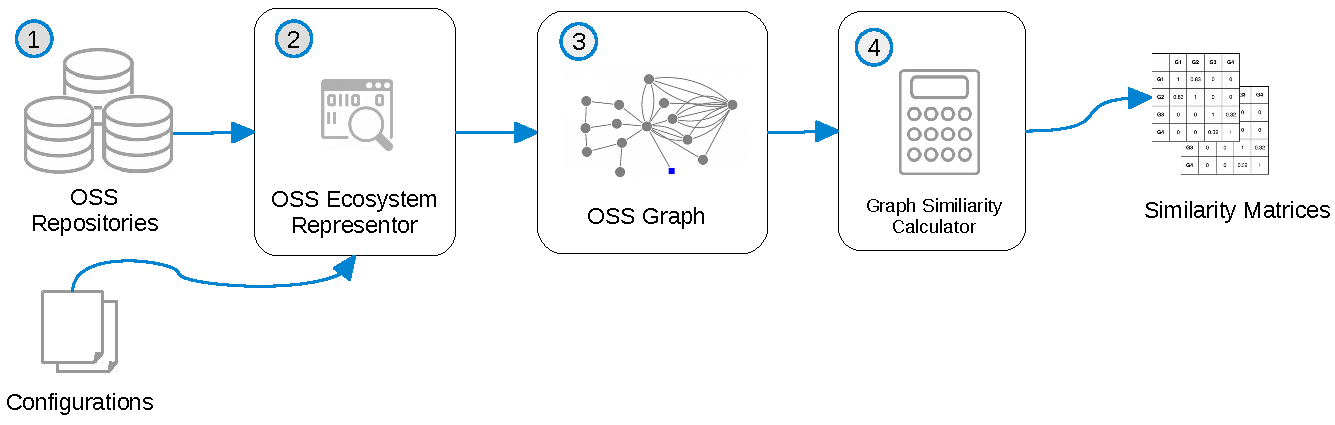
\includegraphics[width=15cm,height=20cm,keepaspectratio]{images/CrossSim.pdf}
 	\caption{The \CrossSim Architecture}
 	\label{fig:CrossSim}
 \end{figure}
 
The architecture of CrossSim is depicted in Figure \ref{fig:CrossSim}: the rectangles represent artifacts, whereas the ovals represent activities that are automatically performed by the developed CrossSim tooling. In particular, the approach imports project data from existing OSS repositories and represents them into a graph-based representation by means of the \emph{OSS Ecosystem Representation} module. Depending on the considered repository (and thus to the information that is available for each project) the graph structure to be generated has to be properly configured. For instance in case of GitHub, specific configurations have to be specified in order to enable the representation in the target graphs of the stars assigned to each project. Such a configuration is ``forge'' specific and specified once, e.g., SourceForge does not provide the star based system available in GitHub. 
 %
The \emph{Graph similarity} module implements the SimRank algorithm \cite{Jeh:2002:SMS:775047.775126} that is applied on the source graph-based representation of the input ecosystems generates matrices representing the similarity value for each pair of input projects. 
 
% \subsection{Graph-based Representation of OSS Ecosystems}
 
We consider the community of developers together with OSS projects, libraries and their mutual interactions as an \emph{ecosystem}. In this system, either humans or non-human factors have mutual dependency and implication on the others. There, several connections and interactions prevail, such as developers commit to repositories, users star repositories, or projects contain source code files, just to name a few. We propose a solution that makes use of graphs for representing relationships in OSS ecosystems. Specifically, the graph model has been chosen since it allows for flexible data integration and facilitates numerous similarity metrics and clustering techniques \cite{Blondel:2004:MSG:1035533.1035557},\cite{Lu2007},\cite{Schaeffer:2007:SGC:2296006.2296057}. All the playing actors and their communications are transformed into a directed graph. Humans and non-human artifacts are represented as nodes and there is a directed edge between a pair of nodes if they interact with each others. The representation model considers different artifacts in a united fashion, taking into account their mutual, both direct and indirect relationships as well as their co-occurrence as a whole. The representation is twofold: First, it incorporates semantic relationships into the graph. Second, it helps combine both low-level and high-level information into a homogeneous representation.
 
 
 
 \begin{figure}[t!]
 	\centering
 	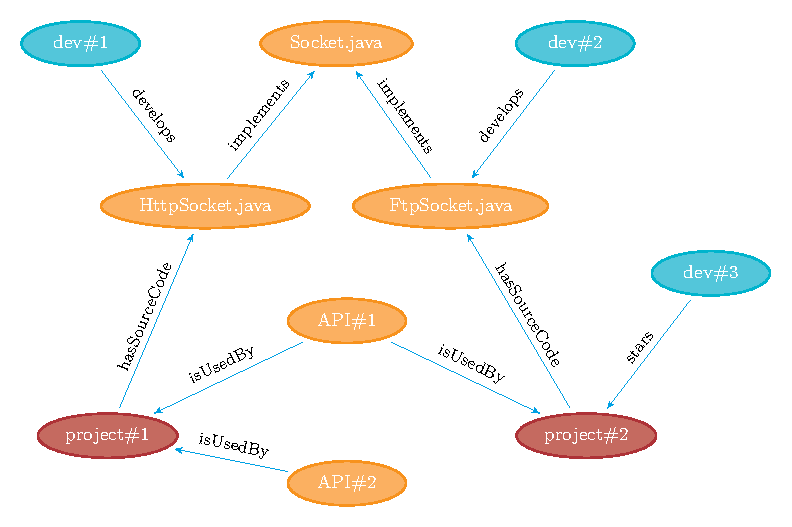
\includegraphics[width=0.60\textwidth]{images/OSSGraph1.pdf}
 	\caption{Sample graph-based representation of OSS ecosystems}
 	\label{fig:OSSGraph1}
 \end{figure}
 
 
To demonstrate the utilization of graphs in an OSS ecosystem, we consider an excerpt of the dependencies for two OSS projects, namely \texttt{project\#1} and \texttt{project\#2} in Figure~\ref{fig:OSSGraph1}. Using dependency information extracted from source code and the corresponding metadata (e.g. coming from the tools developed in by Work Package 2), this graph can be properly built to represent the two projects as a whole. In this figure, \texttt{project\#1} contains code file \texttt{HttpSocket.java} and \texttt{project\#2} contains \texttt{FtpSocket.java} with the corresponding edges being marked with the semantic predicate \texttt{hasSourceCode}. Both source code files implement \texttt{interface\#1} being marked by the semantic predicate \texttt{implements}. \texttt{Project\#1} and \texttt{project\#2} are also connected via other semantic paths, such as API \texttt{isUsedBy} highlighted in Figure~\ref{fig:OSSGraph3}. In practice, an OSS graph is much larger with numerous nodes and edges, and the relationship between two projects can be thought as a sub-graph. 
 
 \begin{figure}[h!]
 	\centering
 	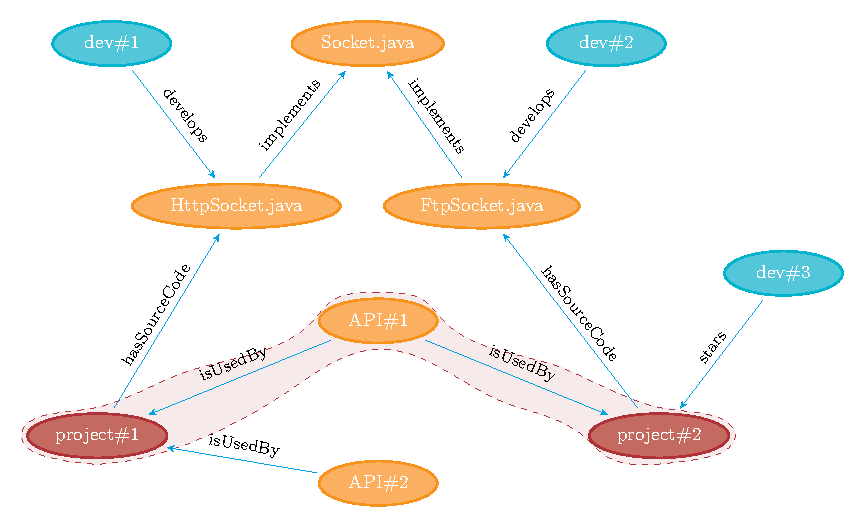
\includegraphics[width=0.60\textwidth]{images/OSSGraph3.pdf}
 	\caption{Similarity between OSS projects with respect to API usage}
 	\label{fig:OSSGraph3}
 \end{figure}
 
 
Based on the graph structure, one can exploit nodes, links and the mutual relationships to compute similarity using existing graph similarity algorithms. To the best of our knowledge, there exist several metrics for computing similarity in graph \cite{Blondel:2004:MSG:1035533.1035557},\cite{Nguyen:2015:CRV:2942298.2942305},\cite{Nguyen:2015:ESP:2740908.2742141}. The graph structure also allows for graph kernel methods, which are an effective way to compute similarity \cite{ODMD14a}. Considering Figure~\ref{fig:OSSGraph1}, we can compute the similarity between \texttt{project\#1} and \texttt{project\#2} with regards to the semantic paths between them, e.g. the two-hop path using \texttt{hasSourceCode} and \texttt{implements} (Figure~\ref{fig:OSSGraph2}), or the one-hop path using API \texttt{isUsedBy}. For example, concerning \texttt{isUsedBy}, the two projects are considered to be similar since with the predicate both projects originate from \texttt{API\#1}. The hypothesis is based on the fact that the projects are aiming at creating common functionalities by using common libraries \cite{McMillan:2012:DSS:2337223.2337267},\cite{6671293}.
 
 
 \begin{figure}[h!]
 	\centering
 	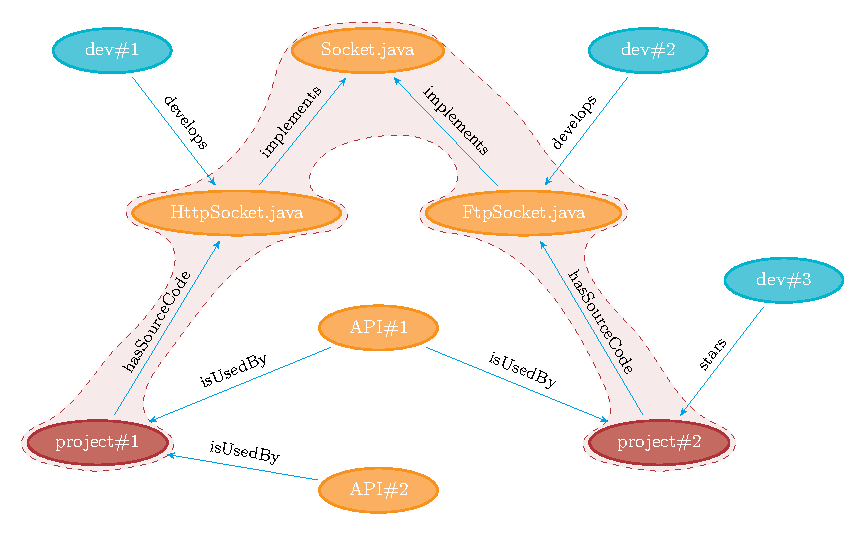
\includegraphics[width=0.60\textwidth]{images/OSSGraph2.pdf}
 	\caption{Similarity between OSS projects with respect to source implementation}
 	\label{fig:OSSGraph2}
 \end{figure}
 
 
The representation allows us to compute similarity between other graph components, e.g. developers. Back to Figure~\ref{fig:OSSGraph1}, though there is no direct connection between \texttt{dev\#1} and \texttt{dev\#2}, their similarity can still be inferred from indirect semantic paths, such as \texttt{develops} and \texttt{implements} which are highlighted in Figure \ref{fig:OSSGraph4}.
 %
If we consider other semantic paths, we see that the two developers have more in common as they both take part in \texttt{project\#1} and \texttt{projects\#2} represented by \texttt{commits}. To a certain extent, the two developers are considered to be similar, although they are not directly connected. In reality, the connection between \texttt{developer\#1} and \texttt{developer\#2} is enforced by further semantic paths and as a result their similarity can be more precisely computed. The similarities between developers can serve as input for a collaborative filtering recommendation system, with which a developer is recommended a list of projects or libraries that similar developers already worked with \cite{Pazzani2007},\cite{Schafer:2007:CFR:1768197.1768208}. This is an invaluable tool in the context of the \projectName project since it is essential to equip developers with recommendation functionalities to help them increase reusability and productivity.
 
 
% \begin{figure}[t!]
% 	\centering
% 	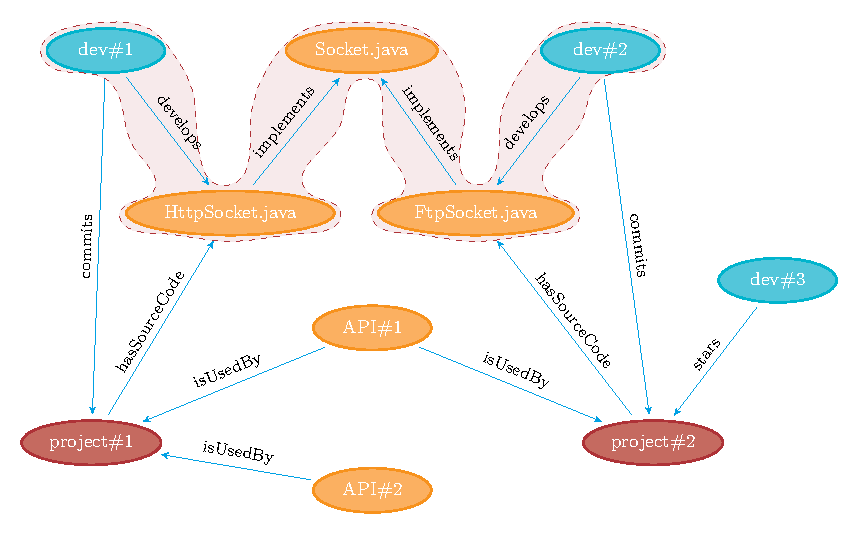
\includegraphics[width=0.60\textwidth]{images/OSSGraph4.pdf}
% 	\caption{Similarity between developers}
% 	\label{fig:OSSGraph4}
% \end{figure}

%\clearpage
 
 
The relationships underpinning the graph-based representations of the simple ecosystems shown in Fig. \ref{fig:OSSGraph1}--\ref{fig:OSSGraph3} are shown in Table~\ref{tab:Representation}. For the first implementation of \CrossSim the relationships $isUsedBy$, $develops$, and $stars$ have been considered. 
 
 
 \begin{table}[h!]
 	\centering
 	\begin{tabular}{|p{5.4cm}|p{8cm}|}  \hline
 		{\bf Relationship} & {\bf Description} \\  \hline
 		\textit{isUsedBy} $\subseteq$ \textit{Dependency}$\times$\textit{Project} & this relationship depicts the reliance of a project on a dependency (e.g., a third-party library). The project needs to include the dependency in order to function. According to \cite{McMillan:2012:DSS:2337223.2337267,6671293} the similarity between two considered projects relies on the dependencies they have in common because they aim at implementing similar functionalities.\\ \hline
 		\textit{develops} $\subseteq$ \textit{Developer} $\times$ \textit{Project} & we suppose that there is a certain level of similarity between two projects if they are built by same developers, as already hypothesized by \cite{Chen:2015:SFD:2684822.2685305}. Thus, this relationship is used to represent the projects that a given user contributes in terms of source code development.\\ \hline
 		\textit{stars} $\subseteq$ \textit{User} $\times$ \textit{Project} & This relationship is inspired by the star event in RepoPal \cite{10.1109/SANER.2017.7884605} to represent GitHub projects that a given user has starred. However, we consider the star event in a broader scope in the sense that not only direct but also indirect connections between two developers is taken into account.\\ \hline
 		\textit{implements} $\subseteq$ \textit{File} $\times$ \textit{File} & It represents a specific relation that can occur between the source code given in two different files, e.g. a class specified in one file implementing an interface given in another file.	\\ \hline
 		\textit{hasSourceCode}  $\subseteq$ \textit{Project} $\times$ \textit{File} & It represents the source files contained in a given project.\\\hline
 	\end{tabular}
 	\caption[Relationships]{Graph Representation of OSS projects}
 	\label{tab:Representation}
 \end{table}
 
%\subsection{Similarity Computation}









\section{Analysis} \label{sec:Analysis}

In this section we present a review on the above mentioned similarity metrics. The review is twofold as follows. First, it helps determine the features that contribute effectively towards similarity computation in OSS projects. Second, it aims at evaluating and identifying the strength as well as the shortcomings of the approaches. Table~\ref{tbl:AlgorithmsAndFeatures} shows a summary of the previously outlined approaches with respect to the features, which are exploited by each technique. In particular, the features shown in Table~\ref{tbl:AlgorithmsAndFeatures}  are:

\begin{itemize}
	\item {\em LOC}: the number of lines of code.
	\item {\em Dep.}: the third-party libraries a project includes.
	\item {\em API calls}: API function calls appear in source code. They are used to build term-document matrices and then to calculate similarities among applications.
	%\item {\em Library}: Third-party libraries used.
	\item {\em Function}: functions and procedures defined in the source code.
	\item {\em Star}: star events in GitHub. Different from the concept of stars or bubbles used in other rating systems like TripAdvisor\footnote{\url{https://www.tripadvisor.com/TripAdvisorInsights/n2640/all-about-your-tripadvisor-bubble-rating}} or Facebook\footnote{\url{https://www.facebook.com/help/548274415377576/}}, stars in GitHub are not used to rate a repository. A developer stars a repository as a way to keep track of it for future reference. In addition, stars are used as a means to thank the repository maintainers for their contribution\footnote{\url{https://help.github.com/articles/about-stars}}.
	\item {\em Timestamp}: the point of time when a user stars a repository. %This feature is used only by RepoPal \cite{10.1109/SANER.2017.7884605}.
	\item {\em Statement}: source code statement.
	\item {\em Readme}: Readme.md or description file, used to describe the functionalities of an open source project. 
	\item {\em Tag}: tags are used by OSS platforms, e.g. SourceForge to classify and characterize an open source project.
	\item {\em Update}: the newest changes made to the app.
	\item {\em Permission}: this feature is available only by mobile apps. It specifies the permission of an app to handle data in a smartphone.
	\item {\em Screenshot}: this feature is available by mobile apps. It is used to compare different apps.
\end{itemize}

As shown in Table~\ref{tbl:AlgorithmsAndFeatures} the techniques that mainly underpin the outlined similarity approaches are:

\begin{itemize}
	\item {\em TDM \& LSA}: Term-Document Matrix \cite{Collobert:2011:NLP:1953048.2078186} and Latent Semantic Analysis \cite{Landauer1998} are generally used in combination to model the relationships between API calls/identifiers and software systems and to compute the similarities between them.
	\item {\em COS}: Cosine Similarity, this technique is widely used in several algorithms for computing similarities among vectors.
	\item {\em JCS}: Jaccard index used for computing similarity between two sets of elements~\cite{jaccard}.
\end{itemize}


Most low-level similarity algorithms (shown as \textit{L} in Table~\ref{tbl:AlgorithmsAndFeatures}) attempt to represent source code (and API calls) in a term-document matrix and then apply SVD to reduce dimensionality. The similarity is then computed as the cosine similarity between feature vectors. Among others, MUDABlue \cite{10.1109/APSEC.2004.69}, CLAN \cite{McMillan:2012:DSS:2337223.2337267}, and CLANdroid \cite{10.1109ICPC.2016.7503721} belong to this category. CLAN includes API calls for computing similarity, whereas, by MUDABlue, every word appearing in source code files is integrated into the term-document matrix. This makes the difference in the performance of the two algorithms in a way that the similarity scores of CLAN reflect better the perception of humans of similarity than those of MUDABlue. %The different 



\begin{landscape}
	\begin{table}[htbp]
		\footnotesize
%		\small
		\centering
		\begin{tabular}{|p{2.5cm}|c|c|c|c|c|c|c|c|c|c|c|}  
			\hline 
			& \textbf{MUDABlue} & \textbf{CLAN} & \textbf{CLANdroid} & \textbf{GPLAG} & \textbf{LibRec} & \textbf{SimApp} & \textbf{AnDarwin} & \textbf{WuKong} & \textbf{TagSim} & \textbf{RepoPal} & \textbf{CrossSim} \\\hline			
			References & \cite{10.1109/APSEC.2004.69} & \cite{McMillan:2012:DSS:2337223.2337267} & \cite{10.1109ICPC.2016.7503721} & \cite{Liu:2006:GDS:1150402.1150522} & \cite{6671293} & \cite{Chen:2015:SFD:2684822.2685305} & \cite{Crussell2013} &  \cite{Wang:2015:WSA:2771783.2771795} & \cite{Lo:2012:DSA:2473496.2473616} & \cite{10.1109/SANER.2017.7884605} & \cite{NDRDSEAA2018} \\\hline
			\multicolumn{12}{|c|}{\bf Features (Modalities)}  \\ \cline{1-12}
			$LOC$ &  &  &  & $\times$ &  &  &  &  &  & &   $\times$ \\\hline
			$Dep.$ &  & $\times$ &  &  &  &  &  &  &  &  & $\times$ \\\hline
			$API$ $Calls$ &  & $\times$ & $\times$ &  & $\times$ &  &  & $\times$ &  & &  $\times$ \\\hline
			$Function$ &  &  &  & $\times$ &  &  &  &  &  &  &  $\times$ \\\hline
			$Star$ &  &  &  &  &  &  &  &   &  & $\times$ &  $\times$ \\\hline
			$Timestamp$ &  &  &  &  &  &  &  &  &   & $\times$  & \\\hline
			$Statement$ & $\times$ &  &  & $\times$ &  &  &  &  &  &   & \\\hline
			$Identifier$  & $\times$ &  & $\times$ &  &  &  &  &  &   &  & \\\hline
			$App. Name$ &  &  &  &  &  & $\times$ &  &  &  & & \\\hline
			$Topic$ &  &  &  &  &  & $\times$ &  &  &  &  & \\\hline
			$Developer$ &  &  &  &  &  & $\times$ &  &  &  &  &  $\times$ \\\hline
			$Readme.md$ &  &  &  &  & $\times$ &  & $\times$ &  & $\times$ & $\times$  & \\\hline
			$Tag$ &  &  &  &  &  &  &  &  & $\times$ &  & \\\hline
			$Update$ &  &  &  &  &  & $\times$ &  &  &   &  & \\\hline
			$Permissons$ &  &  & $\times$ &  &  & $\times$ &  &  &  &  &  \\\hline
			$Screenshot$ &  &  &  &  &  & $\times$ &  &  &  &   & \\\hline
			$Content$ &  &  &  &  &  & $\times$ &  &  &  &  & \\\hline
			$Size$ &  &  &  &  &  & $\times$ &  &  &  &   & \\\hline
			$Reviews$ &  &  &  &  &  & $\times$ &  &  &  & & \\\hline
			$Intent$ &  &  & $\times$ &  &  &  &  &   &   & & \\\hline
			$Sensors$ &  &  & $\times$ &  &  &  &  &  &   & & \\\hline
			
			\multicolumn{12}{|c|}{\bf Used Techniques} \\ \cline{1-12}
			$TDM \& LSA$ & $\times$ & $\times$ & $\times$ &  &  &  &  &  &   &  & \\\hline
			%$LSA$ & $\times$ & $\times$ & $\times$ &  &  &  &  &  &   &  \\ \hline
			$COS$ & $\times$ & $\times$ & $\times$ &  & $\times$ & $\times$ &  & $\times$  &  $\times$ & $\times$  & \\\hline
			$JCS$ &  &  &  &  &  &  & $\times$ &  &  & $\times$ & \\\hline
			
			\multicolumn{12}{|c|}{\bf Category}  \\ \cline{1-12}
			$High/Low$ $Sim$ & L & L & L & L & L & H & H & L & H  & H  & L \& H \\\hline
			
		\end{tabular}
		\caption{Summary of the similarity algorithms and their features}
		\label{tbl:AlgorithmsAndFeatures}
	\end{table}	
\end{landscape}


In contrast, high-level similarity techniques (shown as \textit{H} in Table~\ref{tbl:AlgorithmsAndFeatures}) do not consider source code for similarity computation. They characterize software by exploiting available features such as descriptions, user reviews, and \code{README.MD} file. The similarity is computed as the cosine similarity of the corresponding feature vectors. For computing similarity between mobile applications, other specific features such as images and permissions are also incorporated. A current trend in these techniques is to exploit textual content to compute similarity, e.g. in AppRec \cite{confairsBhandariSDJ13}, SimApp \cite{Chen:2015:SFD:2684822.2685305}, TagSim \cite{Lo:2012:DSA:2473496.2473616}. A main drawback with this approach is that, same words can be used to explain different requirements or the other way around, the same requirements can be described using different words \cite{10.1109/APSEC.2004.69}. So it might be the case that two textual contents with different vocabularies still have a similar description or two files with similar vocabularies contain different descriptions. The matching of words in the descriptions as well as source code to compute similarity is considered to be ineffective as already stated in \cite{McMillan:2012:DSS:2337223.2337267}. To overcome this problem, the application of a synonym dictionary like WordNet \cite{Miller:1995:WLD:219717.219748} is beneficial. Furthermore, the utilization TDM and LSA in textual contents is proven to be effective as LSA helps consider latent semantic relationships. Nevertheless, there is still a problem with the approaches like RepoPal where readme file is used for similarity computation, since in general the descriptions for software projects are written in different languages. According to our observation in GitHub, \code{README.MD} files are written in various languages, \eg not only English but also Japanese, Korean, or Chinese. And the comparison of a readme file in Japanese with one in English should yield dissimilarity, even though two projects may be similar. SimApp \cite{Chen:2015:SFD:2684822.2685305} is the only technique that attempts to combine several high-level information into similarity computation. It eventually applies a machine learning algorithm to learn optimal weights. The approach is promising, nevertheless it is only applicable in the presence of a decent training dataset, which is hard to come by in practice.

\CrossSim is an approach that attempts to combine both low-level and high-level information in computing similarities. The approach integrates implicit semantic relationships and intrinsic dependencies among different users, repositories, source code. Thus, it is able to incorporate new features, on the fly, into the similarity computation without modifying the internal design. \CrossSim is expected to improve the overall performance of the similarity computation and thus the quality of the eventual recommendations. In the next chapter, we are going to introduce our implementation and evaluation of \CrossSim with respect to some notable tools, \ie \MUDABlue, \CLAN, and \RepoPal.


%We aim to design a representation model that integrates semantic relationships among various artifacts and
% By considering all artifacts in a mutual relationship, we aim at improving the overall performance of the similarity computation and
% In the next section, we propose a similarity model that attempts to exploit effectively the rich metadata infrastructure provided by the \projectName Knowledge Base by trying to incorporate various features in computing similarity. Afterwards, we present an initial evaluation on a real dataset collected from GitHub to demonstrate the performance of our approach. 
%in computing similarities and this seems to be beneficial to the context of OSS repositories. 
%should be highly beneficial to the context of OSS repositories. various input information, We hypothesize that combining 
%%==================================Highlight the difference that CrossSim can make, the flexibility==================================
%Most approaches are either low-level or high-level similarity. We see that either a low-level or a high-level similarity metric is able to deal with a certain set of features, they cannot work given that more features are available for similarity computation. In this sense, these metrics can only be applied in a limited context. They can be applied in a limited context, whereas CrossSim gives more flexibility. An approach that is more flexible and overcomes the limitations. The flexibility of. 

%In the next section, we present a novel approach for computing software similarities by allowing one to incorporate various features into the computation.






















%In summary, by reviewing other additional similarity metrics \cite{Crussell2013,10.1109ICPC.2016.7503721,Liu:2006:GDS:1150402.1150522,xia:tag:2013} which cannot be presented here due to space limitation, we have seen that they normally deal with either low-level or high-level similarity. % and to pave the way for . 
%We are convinced that combining various input information in computing similarities is highly beneficial to the context of OSS repositories. We aim to design a representation model that integrates semantic relationships among various artifacts and the model is expected to improve the overall performance of the similarity computation.% and to pave the way for . 


%$SimApp$ \cite{Chen:2015:SFD:2684822.2685305} is the only technique that attempts to combine several high-level information into similarity computation. The approach is promising, nevertheless it is only applicable in the presence of a decent training dataset, which is hard to come by in practice. 
%
%
%\section{A Comprehensive Analysis on the Similarity Metrics} \label{sec:Analysis}
%
%In this section we present a review on the above mentioned similarity metrics. The review is twofold as follows. First, it aims at evaluating and identifying the strength as well as the shortcomings of the approaches. Second, it helps determine the features that contribute effectively towards similarity computation in OSS projects.
%
%Most low-level similarity algorithms attempt to represent source code, API calls in a term-document matrix and then apply SVD to reduce dimensionality. The similarity is then computed as the cosine similarity between feature vectors. Among others, $MUDABlue$ \cite{10.1109/APSEC.2004.69}, $CLAN$ \cite{McMillan:2012:DSS:2337223.2337267}, and $CLANdroid$ \cite{10.1109ICPC.2016.7503721} belong to this category. $CLAN$ includes API calls for computing similarity, whereas, by $MUDABlue$, every word appearing in source code files is integrated into the term-document matrix. This makes the difference in the performance of the two algorithms in a way that the similarity scores of $CLAN$ reflect better the perception of humans of similarity than those of $MUDABlue$. %The different 
%
%In contrast, high-level similarity techniques do not consider source code for similarity computation. They characterize software by exploiting available features such as descriptions, user reviews, readme file. The similarity is computed as the cosine similarity of the corresponding feature vectors. For computing similarity between mobile applications, other specific features such as images and permissions are also incorporated. A current trend in these techniques is to exploit textual content to compute similarity, e.g. in $AppRec$ \cite{confairsBhandariSDJ13}, $SimApp$ \cite{Chen:2015:SFD:2684822.2685305}, $TagSim$ \cite{Lo:2012:DSA:2473496.2473616}. A main drawback with this approach is that, same words can be used to explain different requirements or the other way around, the same requirements can be described using different words \cite{10.1109/APSEC.2004.69}. So it might be the case that two textual contents with different vocabularies still have a similar description or two files with similar vocabularies contain different descriptions. The matching of words in the descriptions as well as source code to compute similarity is considered to be ineffective as already stated in \cite{McMillan:2012:DSS:2337223.2337267}. To overcome this problem, the application of a synonym dictionary like WordNet \cite{Miller:1995:WLD:219717.219748} is beneficial. Furthermore, the utilization TDM and LSA in textual contents is proven to be effective as LSA helps consider latent semantic relationships. Nevertheless, there is still a problem with the approaches like $RepoPal$ where readme file is used for similarity computation, since in general the descriptions for software projects are written in different languages. According to our investigations on GitHub, projects include \emph{readme.md} in various languages, such as Japanese, Korean, and Chinese. And the comparison of a readme file in Japanese with one in English should yield dissimilarity. $SimApp$ \cite{Chen:2015:SFD:2684822.2685305} is the only technique that attempts to combine several high-level information into similarity computation. It eventually applies a machine learning algorithm to learn optimal weights. The approach is promising, nevertheless it is only applicable in the presence of a decent training dataset, which is hard to come by in practice.
%
%We are convinced that combining both low-level and high-level information in computing similarities should be highly beneficial to the context of OSS repositories. We expect a representation model that integrates implicit semantic relationships and intrinsic dependencies among different users, repositories, source code. By considering all artifacts in a mutual relationship, we aim at improving the overall performance of the similarity computation. In the next section, we propose a similarity model that attempts to exploit effectively the rich metadata infrastructure provided by \projectName Knowledge Base by trying to incorporate various features in computing similarity. Afterwards, we present an initial evaluation on a real dataset collected from GitHub to demonstrate the performance of our approach. Apart from $RepoPal$, some additional similarity metrics are derived and work as baselines for comparison. 
%




	\clearpage
	%	
	%	
	\chapter{Implementation}
	\label{sec:Implementation}
	%%%%%%%%%%%%%%%%%%%%%%%%%%%%%%%%%%%%%%%%%%%%%%%%%%%%%%%%%%%%%%%%%%%%%%%%%%%%%%%%%%%%%%%%%%%%%



\section{Overview}

In this chapter we provide a description on the implementation for different similarity tools. In particular, we will discuss about \MUDABlue, \CLAN, \RepoPal and \CrossSim. As explained before, the purpose is to provide a baseline to evaluate CrossSim, so it's mandatory to have a precise idea of what these approaches are and how does they work. Concerning MudaBlue and Clan, we will discuss about their rationale, showing also their original results, then we will show how we reimplemented such approaches from an high-level point of view.


\section{MUDABlue}

The first procedure analysed was MUDABlue, unfortunately none implentation was available on the web, so i reimplemented it from scratch. The MUDABlue method is an automatc categorizaton method of a large collecton of software systems. MUDABlue method does not only categorize sooware systems but also determines categories from the software systems collection automatigcally. MUDABlue has three major aspects: 1) it relies on no other information than the source code, 2) it determines category sets automatically, and 3) it allows a software system to be a member of multiple categories. Since we were interested only in the evaluation of the similarity we discarded the phases related to clusterization and categorization.

The MUDABlue approach can be briefly summarized in 7 steps, as the following image depicts:

\begin{figure}[!h]
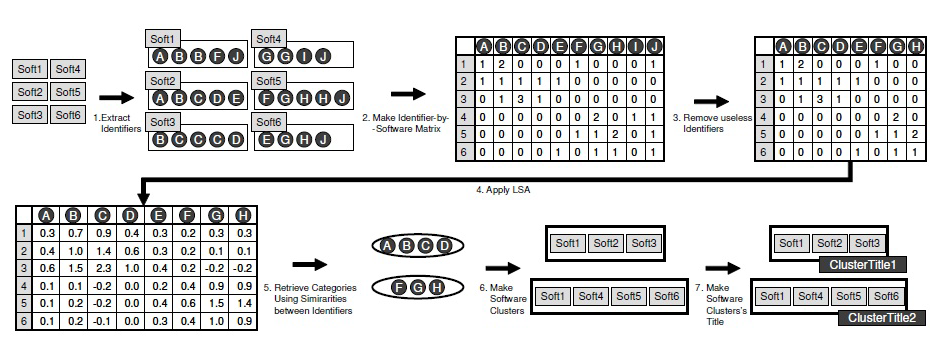
\includegraphics[width=15cm,height=20cm,keepaspectratio]{images/Mudablue1.png}
\centering
\caption{MUDABlue phases.}
\end{figure}

\subsection{Exctract Identifiers}
With identifier we are talking about relevant strings that can allow to characterize a document. In this phase each repository is scanned in order to find the target files, and for each of them the identifiers are exctracted, avoiding adding useless items such as comments. The dataset was a 41C projects gathered from SourceForge.

\subsection{Create identifier-by-software matrix}
As stated before, the main item to work with is the term-document matrix, in this case we count how many times each term appears in each file for all the projects. The result is matrix \textbf{m x n} with m terms and n projects.

\subsection{Remove useless identifiers}
From the matrix we remove all the useless terms, that is all the terms that apperas in just one repository, considered a specific terms, and all the terms that appears in more than 50\% of the repositories, considered as general terms.

\subsection{Apply the LSA}
Once the matrix is ready con be worked, the \emph{SVD} procedure is applied and then the LSI. As explained before [NOTE] the \emph{SVD} procedure decompose the original matrix in 3 other matrices. When we multiply back these matrices we use a rank reducted version of the S matrix in order to generete the final one. The authors didn't provide us any details about their final rank value, so we tested many values and eventually selected one.

\subsection{Apply the Cosine Similarity}
By using the cosine similarity method, we compare each repository vector with all the others and eventually getting an \textbf{n x n} matrix, in which is expressed the similarity of all the repository couple, with a value \emph{[0.0-1.0]}. Thereafter, the cluster analysis is applied using calculated similarities. 

\subsection{Categorization}
Make software clusters from identifier clusters. From each identifier clusters, the software systems that contain one or more identifiers in the cluster are retrieved. The last step is to make software clusters’ titles. This can be done by summing all identifier-vectors comprised in the identifier cluster and then consider the ten identifiers that got the highest value in the summation vector.

\subsection{Results}
The experimentation was conducted on a corpus of $41$ \emph{C} projects, taken form SourceForge belonging to $5$ categories.
Developers used \emph{precision} and \emph{recall} as criteria, defined as follows:

\begin{equation}
Precision = \frac{\sum_{s\in S}\text{precision}_{soft}\text{(S)}}  {\mid S \mid}
\end{equation}

\begin{equation}
Recall = \frac{\sum_{s\in S}\text{recall}_{soft}\text{(S)}}  {\mid S \mid}
\end{equation}

\begin{equation}
Precision_{soft}\text{(s)} = \frac{\mid C_\text{MudaBlue}\text{(s)} \cap C_\text{Ideal}\text{(s)} \mid}  {\mid C_\text{MudaBlue}\text{(S)} \mid}
\end{equation}

\begin{equation}
Recall_{soft}\text{(s)} = \frac{\mid C_\text{MudaBlue}\text{(s)} \cap C_\text{Ideal}\text{(s)} \mid}  {\mid C_\text{Ideal}\text{(s)} \mid}
\end{equation}

where $C_\text{MudaBlue}\text{(s)}$ is a set of categories containing software s, generated by MUDABlue, $C_\text{Ideal}\text{(s)}$ is a set of categories containing software \emph{s}, determined manually by the experimenters. In both of the criteria, the larger value,
the better result.

%\clearpage


%%%%%%%%%%%%%%%%%%%%%%%%%%%%%%%%%%%%%%%%%%%%%%%%%%%%%%%%%%%%%%%%%%%%%%%%%%%%%%%%%%%%%%%%%%%%%

\section{CLAN:  Closely reLated ApplicatioNs}

\textit{CLAN} \cite{McMillan:2012:DSS:2337223.2337267} is an approach for automatically detecting similar Java applications by exploiting the semantic layers corresponding to packages class hierarchies. \textit{CLAN} works based on the document framework for computing similarity, semantic anchors, e.g. those that define the documents' semantic features. Semantic anchors and dependencies help obtain a more precise value for similarity computation between documents. The assumption is that if two applications have API calls implementing requirements described by the same abstraction, then the two applications are more similar than those that do not have common API calls. The approach uses API calls as semantic anchors to compute application similarity since API calls contain precisely defined semantics. The similarity between applications is computed by matching the semantics already expressed in the API calls.

The process consist of 12 steps here graphically reported.

\begin{figure}[!h]
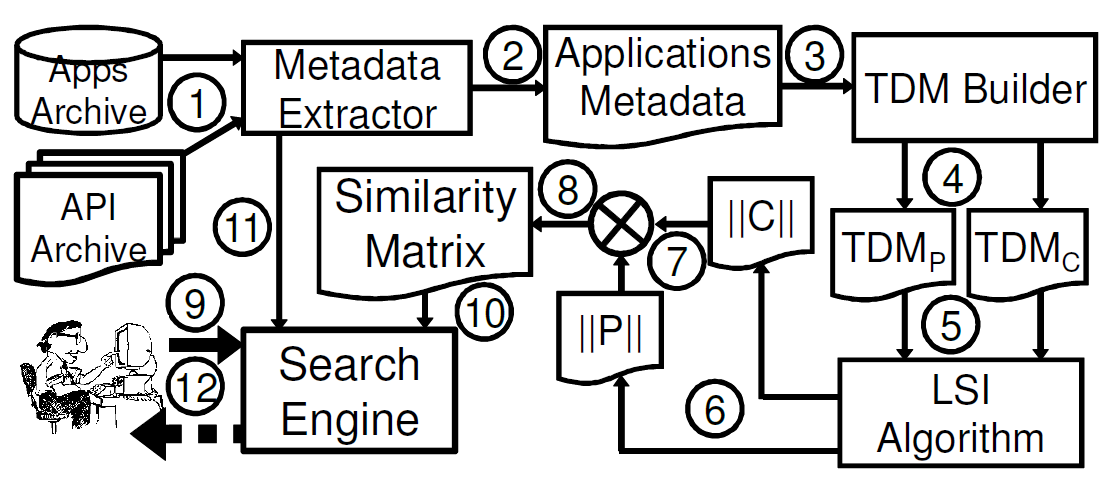
\includegraphics[width=0.80\textwidth]{images/Clan.png}
\centering
\caption{CLAN phases.}
\end{figure}



\subsection{Terms Extraction}
Steps from 1 to 3 can be merged together since are related to extraction of terms from the repositories.
As stated before, an important concept is that terms extracted are only API calls, this means that all other things present in a piece of code are discarded, for example all the variables or the function declaration and invocation. Furthermore these API calls belong only to the JDK, in such a way also the calls to any other external library are discarded. This idea is also applied in the extraction of the import declaration, focus only on the JDK packages import.
The result of this process will be an ordered set of data, representing the occurrencies of any Package;Class for all the projects.

\subsection{TDMs Creation}
Once the dataset as been created, is reorganized in TDMs. Here two different matrices are created, one for the Classes and one for the Packages. Class-level and package-level similarities are different since applications are often more similar on the package level than on the class level because there are fewer packages than classes in the JDK. Therefore, there is the higher probability that two applications may have API calls that are located in the same package but not in the same class.

\subsection{LSI Procedure}
The paper refers to LSI procedure, Latent Semantic Indexing[dumais2], but the term are synonym, so from here on, we will refer as Latent Semantic Analysis LSA.

\subsection{Apply the Cosine Similarity}
As for Mudablue, we will apply the cosine similarity to the matrix got from the LSA procedure.

\subsection{Sum of the matrices}
The 2 matrices are summed, but before are multplied by a certain value. Since the values for the entries in the 2 matrices are between 0.0 and 1.0 a simple sum could result in a value over 1.0, by this multiplication these values are reducted in order to be summed togheter but still maintaining the logical meaning. The authors chosen 0.5, also we, since is a good value to equal distribute the weight of the packages and method calls.The sum of this value is 1.0, and can span from 0.1 to 0.9 for each matrix, is clear that more is high on a matrix, more is important the values that we are considering from such matrix.

\subsection{Final similarity matrix}
Once the matrix is ready, the system will use it to answer the query of users, from such  matrix the system will retrieve the common projects ordered by rank.

\subsection{Results}
The developers used a corpus of $8310$ projects from SourceForge, for a total of $114146$ API calls. The evaluation method was similar to our, a user study with a group of 33 student of University of Illinois at Chicago with at least 6 months of java experience. Their main task was to examine the retrieved applications and to determine if they are relevant to the tasks and the source application. Each participant accomplished this step individually, assigning a confidence level, C, to the examined applications using a four-level Likert scale.


%\begin{figure}[!h]
%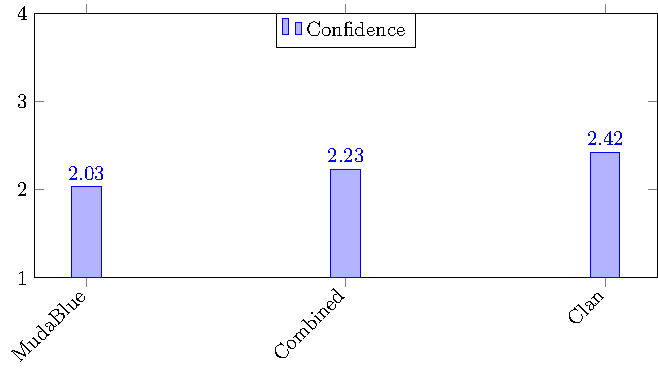
\includegraphics[width=10cm,height=15cm,keepaspectratio]{images/ConfidenceClan.pdf}
%\centering
%\caption{Confidence Comparison Original Clan}
%\label{fig:ConfidenceClan}
%\end{figure}
%
%\begin{figure}[!h]
%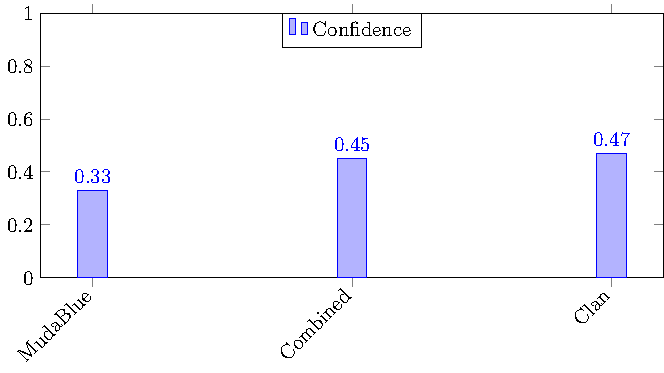
\includegraphics[width=10cm,height=15cm,keepaspectratio]{images/PrecisionClan.pdf}
%\centering
%\caption{Precision Comparison Original Clan}
%\label{fig:PrecisionClan}
%\end{figure}


%Figure \ref{fig:ConfidenceClan} and figure \ref{fig:PrecisionClan} reports the mean of the results they got from the students. As you can see the Clan approach performs better than MudaBlue. Since Similarity Matrices of MUDABlue and CLAN have the same dimensions, it is possible to construct a combined matrix whose values are the average of the values of the MUDABlue and CLAN matrix elements at the corresponding position. [nota e chiedere]

%\clearpage


%%%%%%%%%%%%%%%%%%%%%%%%%%%%%%%%%%%%%%%%%%%%%%%%%%%%%%%%%%%%%%%%%%%%%%%%%%%%%%%%%%%%%%%%%%5  

\section{RepoPal: Exploiting Metadata to Detect Similar GitHub Repositories}\label{sec:repopal}

In contrast to many previous studies that are generally based on source code \cite{10.1109/APSEC.2004.69},\cite{Liu:2006:GDS:1150402.1150522},\cite{McMillan:2012:DSS:2337223.2337267}, \textit{RepoPal}  \cite{10.1109/SANER.2017.7884605} is a high-level similarity metric and takes only repositories metadata as its input. With this approach, two GitHub repositories are considered to be similar if:

\begin{itemize}
	\item[i)] They contain similar readme files;
	\item[ii)] They are starred by users of similar interests;
	\item[iii)] They are starred together by the same users within a short period of time. 
\end{itemize}

Thus, the similarities between GitHub repositories are computed by using three inputs: readme file, stars and the time gap that a user stars two repositories. Considering two repositories $ r_{i} $ and $ r_{j} $, the following notations are defined: 

\begin{itemize}
	\item $ f_{i} $ and $ f_{j} $ are the readme files with $ t $ being the set of terms in the files; 
	\item $ U(r_{i}) $ and $ U(r_{j}) $ are the set of users who starred $ r_{i} $ and $ r_{j} $, respectively; 
	\item $ R(u_{k}) $ is the set of repositories that user $ u_{k} $ already starred.  
\end{itemize}

There are three similarity indices as follows:

\paragraph{Readme-based similarity} 

The similarity between two readme files is calculated as the cosine similarity between their feature vectors $\vec{f_{i}}$ and $\vec{f_{j}}$: 

\begin{equation}
sim_{f}(r_{i},r_{j})=CosineSim(\vec{f_{i}},\vec{f_{j}})
\end{equation}
\clearpage

%%%%%%%%%%%%%%%%%%%%%%%%%%%%%%%%%%%%%%%%%%%%%%%%%%%%%%%%%%%%%%%%%%%%%%%%%%%%%%%%%%
\section{CrossSim}

Since the purpose of this thesis is to provide implementation and data to validate CrossSim approach, is useful to explain in detail it.
So this section we are going to present CROSSSIM (Cross Project Relationships for Computing Open Source Software Similarity), an approach that makes use of graphs for representing different kinds of relationships in the OSS ecosystem. In particular, with the adoption of the graph representation, we are able to transform the relationships among non-human artifacts, e.g. API utilizations,
source code, interactions, and humans, e.g. developers into a mathematically computable format, i.e. one that facilitates various types of computation techniques.







%%%%%%%%%%%%%%%%%%%%%%%%%%%%%%%%%%%%%%%%%%%%%%%%%%%%%%%%%%%%%%%%%%%%%%%%%%%% 
\section{System Description}
In this section we want to explain our work and what we have done. In order to do this we will use some UML diagram plus a generich high level architecture diagram.
\begin{figure}[!h]
	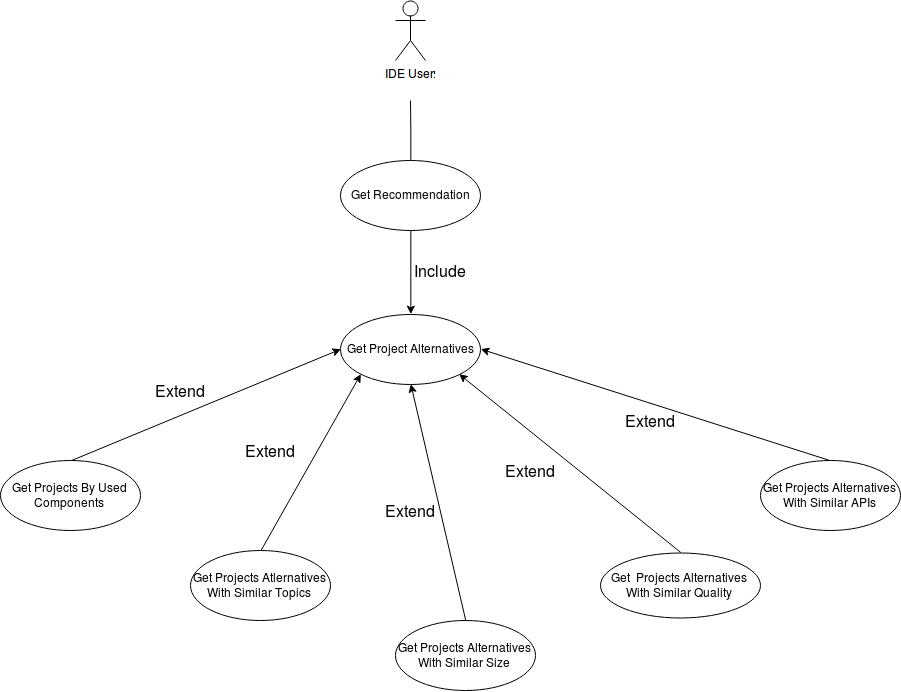
\includegraphics[width=15cm,height=20cm,keepaspectratio]{images/UseCaseDiagram.png}
	\caption{Use Case Diagram}
	\label{fig:UseCase}
\end{figure}
This image, exctracted from CrossSim documentation depicts how a similarity calculator fits inside a real project.
It is clear that in order to provide a meaningful recommendation, it is mandatory to have a similarity calculator better as possible since all the functionality extending the \emph{GetProjectAlternatives} use case, rely on some similarity computation.



\subsection{Component Point of View}
\begin{figure}[!h]
	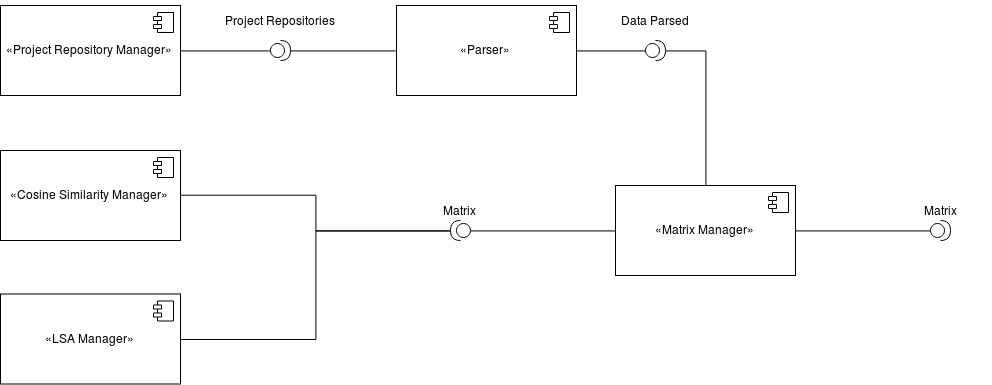
\includegraphics[width=15cm,height=20cm,keepaspectratio]{images/ComponentDiagram.png}
	\caption{Component Diagram}
	\label{fig:Component}
\end{figure}
As you can see there are 5 main components:
\begin{itemize}
	\item Project Repository manager: this is the component who provide the repositories and who manage the file system.
	\item Parser: this component analyzes all the \emph{.java} files in order to retrieve the keywords to create the term-document matrix. As stated before we search for the \emph{JDK} related imports and methods for Clan and any imports, method, variables and field variables for MudaBlue.
	\item Matrix Manager: the matrix manager is the central component, in the sense that manages the creation of the term-document matrix, but not only, it coordinates all the matrices "roaming" during the process. For example the term-document matrix can't be analzed as it is by the SVD component, it requires a rework before.
	\item LSA Manager: here all the operations concerning the Latent Semantic Analsys occurs, from the low-rank matrix reduction to the Singular Value Decomposition.
	\item Cosine Similarity Manager: once the LSA completes his work we can apply the cosine similarity to get the final version of the matrix.
\end{itemize}

\begin{figure}[!h]
	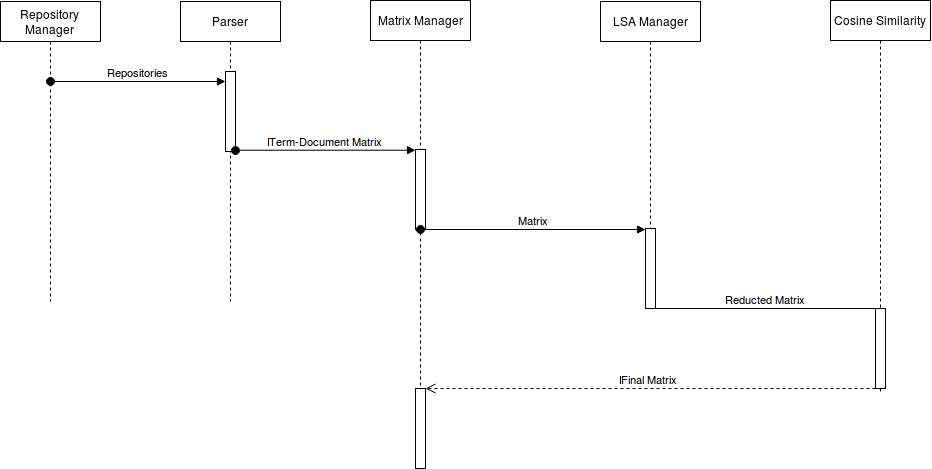
\includegraphics[width=15cm,height=20cm,keepaspectratio]{images/SequenceDiagram.png}
	\caption{Sequence Diagram}
	\label{fig:Sequence}
\end{figure}

In the figure \ref{fig:Sequence} we can see the sequence diagram.
When the process starts, the repository manager analyzes the file system in order to provide all the repositories to be analyzed. It also check if the parsing has been occurred before to such repositories, this is due the extremely high consumption of memory, so we splitted the phases in two moments.\\
When we know what are the repositories to be analyzed we can start, as explained before for MudaBlue and Clan the terms are different, but we still use the same library in both cases \emph{Java Parser}.\\
The outcome will be a term-document matrix worked by the Latent Semantic Analysis manager.
First of all we invoke the \emph{commons math} for decomposing the matrix, then we can multiply them back in order the get the LSA matrix.\\
At this stage we just need to take the matrix and then apply the cosine similarity, for each vector of the matrix we calculate the cosine with all the others vectors. In this way we will get a final matrix of \emph{580 x 580}.
The final matrix can be taken for further analysis or anything that we need.




%\clearpage

\subsection{Description}
\begin{figure}[!h]
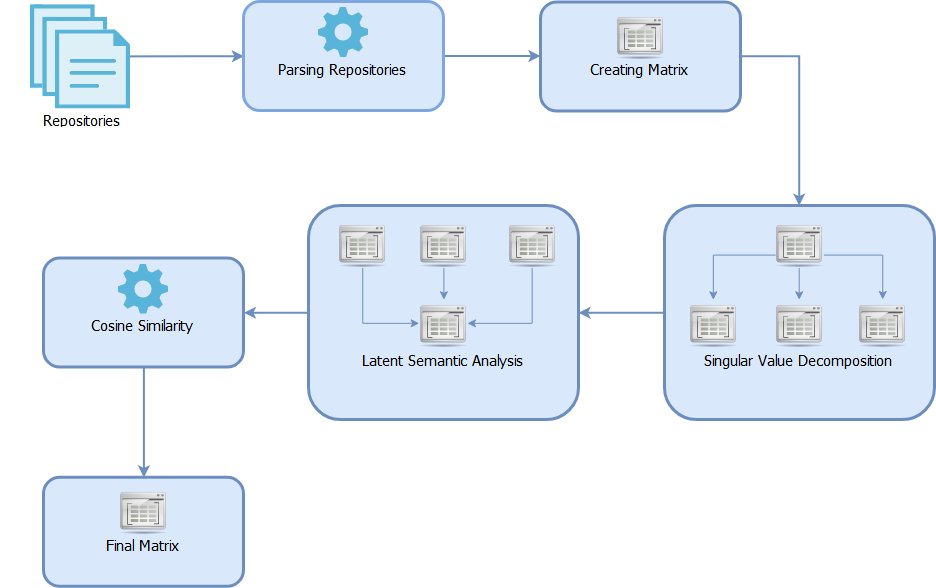
\includegraphics[width=15cm,height=20cm,keepaspectratio]{images/Architecture.png}
\caption{System Structure}
\end{figure}

In this image is depicted the general architecture of the implemented systems, as you can see the systems share the same architecture with some differences that will be discussed later.
As you can see, the process consist of 7 steps.
\begin{itemize}
 \item Retrieving the dataset, in this case a folder with all 580 repositories.
 \item All these repositories are analyzed, and any \emph{.java} file is parsed.
 \item For each repository a vector that contains all the frequencies for each term found is created, and then added in a matrix. 
 \item The SVD procedure, decomposing the matrix in other 3.
 \item The matrices are multiplied back to realize the LSA procedure.
 \item For each vector, we count the cosine similarity with all the others.
 \item Now we have the final matrix, where any repositories is compared to all the others.
\end{itemize} 




\subsection{System Details}

\begin{figure}[!h]
	\centering
	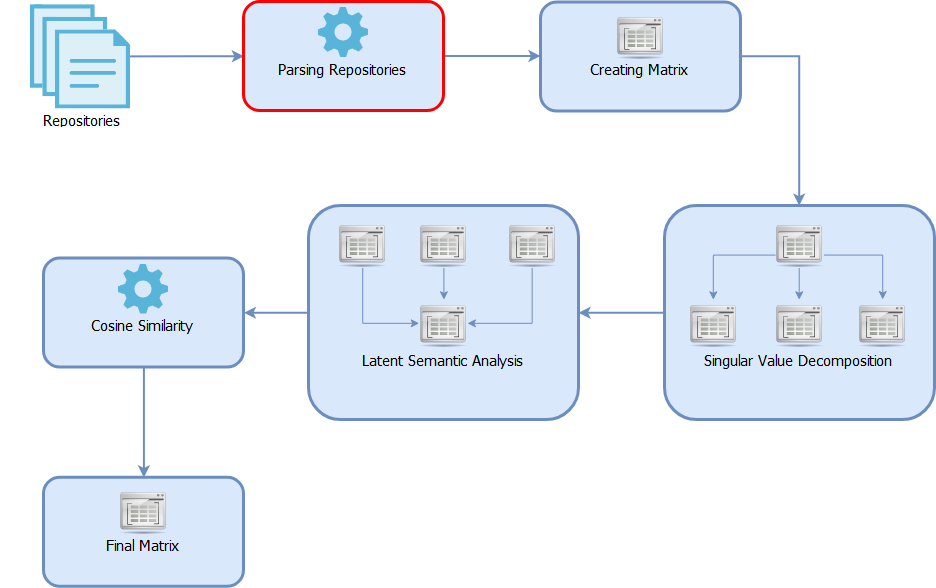
\includegraphics[width=0.8\textwidth]{images/Architecture1.png}
	\caption{Parsing}
\end{figure}


Parsing: The first step is clearly parsing the java files of the 580 repositories. We used the javaparser library to directly access
the main components of the files (import and method invocation for CLAN, import, method declaration, variables and field variables for MudaBlue). For each repository we created a relative .txt file containing the frequencies, for the CLAN approach such terms are filtered by searching only the terms belonging to the Java JDK. All these terms are merged in another file, called mainlist.txt which is used to avoid reps. The idea is parsing the files and compare with the mainlist.txt to add new terms, and then count, for each terms how many times appears inside the files. So the result will be a vector of numbers.

\begin{figure}[!h]
	\centering
	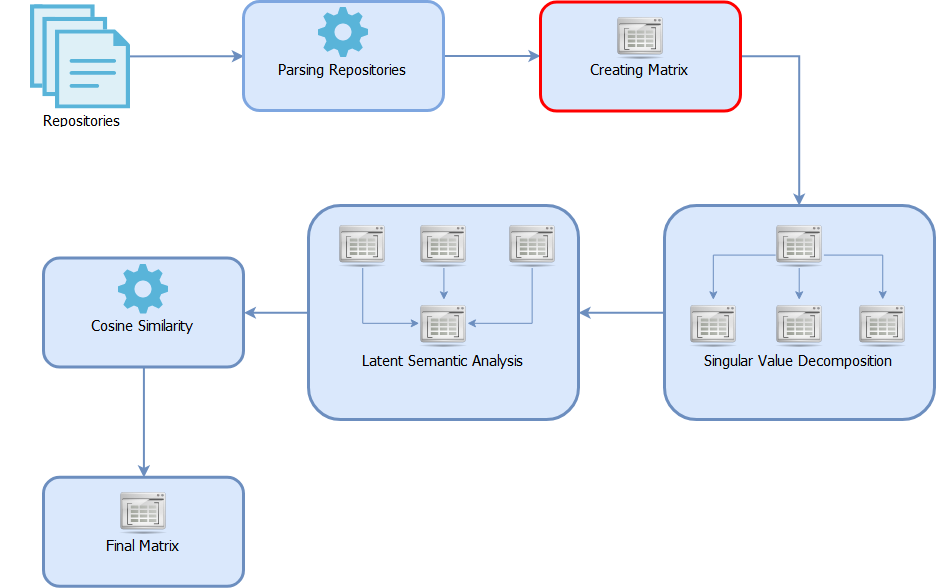
\includegraphics[width=0.8\textwidth]{images/Architecture2.png}
	\caption{Matrix Creation}
\end{figure}


Matrix Creation: Once all the repositories are analyzed we can procede in creating the term-document matrix. The matrix is created using the library \emph{apache commons math3} and in particular these components:
\begin{itemize}
\item ArrayRealVector.
\item RealMatrix.
\item RealVector.
\end{itemize}
Each files contains only his own terms naturally, so the idea is, once the parsing process is done, to count how many terms we have and then, adding many zeros as many terms are missing. To clarify, imagine that we have 3 documents \emph{A,B,C} for 10 different terms.
Now if we examine the document A, we might discover 4 terms, this means that the other 6 terms are missing here, so can be marked as 0. 
For the document B, we might find out 2 new terms, and so on.


\begin{figure}[!h]
	\centering
	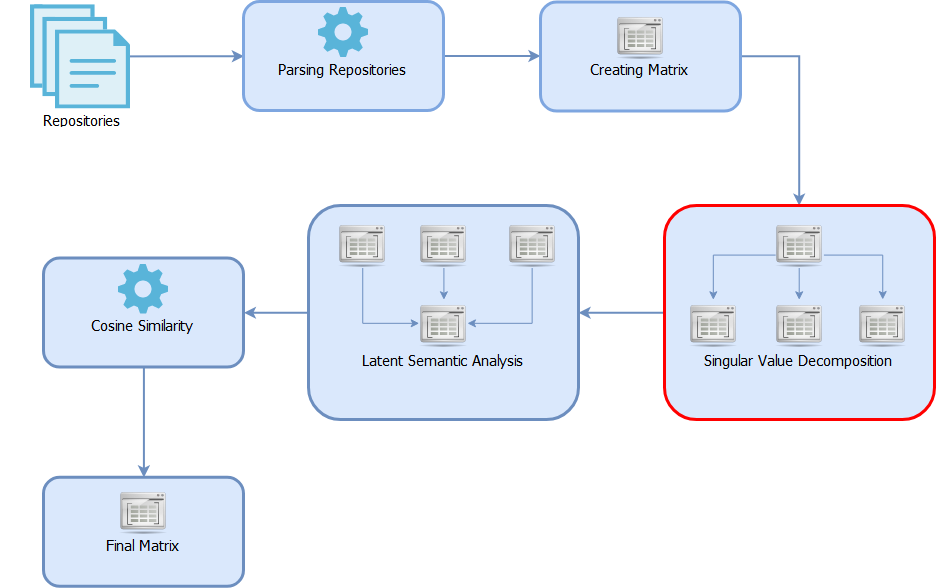
\includegraphics[width=0.8\textwidth]{images/Architecture3.png}
	\caption{Singular Value Decomposition}
\end{figure}

SVD: As stated before the svd operation consist in decomposing the main matrix in other 3.

\begin{equation}
A_{mn}=U_{mm}S_{mn}V_{mn}^{T}
\end{equation}

in which

\begin{itemize}
	\item $U_{mm}$: Orthogonal matrix.
	\item $S_{mn}$: Diagonal matrix.
	\item $V_{mn}^{T}$: The transpose of an orthogonal matrix.
	\item $X$: Low Rank matrix.
\end{itemize}

Such operation are provided by \emph{math3 linear SingularValueDecomposition}.
So we invoke the methods passing as parameter the term-document matrix.
As you can see this operation was already available in the library, so we just retrieved the results of the operation.

\begin{figure}[!h]
	\centering
	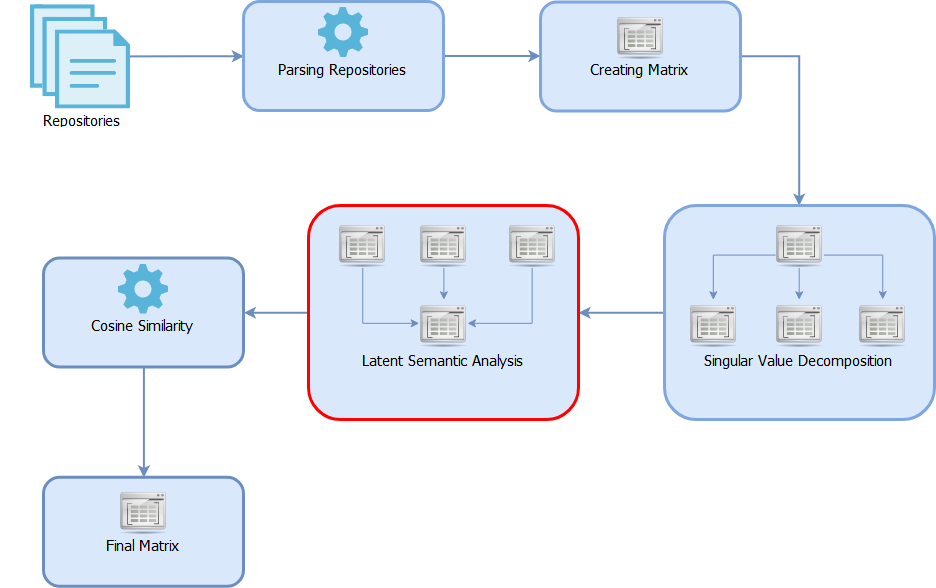
\includegraphics[width=0.8\textwidth]{images/Architecture4.png}
	\caption{Latent Semantic Analysis}
\end{figure}

LSA: Unfortunately an implementation of Latent Semantic Analysis wasn't available, so we re-implemented from scratch.
Basically we multiplied the 3 matrix provided by the \emph{SVD} procedure, the important point is the value \emph{k} for the reduced rank, we selected a value of total $\frac{repository}{2}$. As explained in the Dumais paper, this value should be selected empirically. 
Here we got a very big issue since the
$Memory\,in\,gigabytes\,=\,\frac{(columns*rows*8)}{(1024*1024*1024)}$ is required for a matrix, for MudaBlue we got an amount of 700000 distinct terms for a total of 3GB of dedicated memory just for matrix, without cosidering any kind of operation. This is due to the fact that MudaBlue considers many different terms from a file. Clan instead, focusing only on the the import and method that belongs to the \emph{JDK}, reduced greatly the number of distinct terms. The main solution was to increase the available memory for eclipse up to 8GB. Even though this memory space, we got many crashes, so we spent some time in refactoring the code to save memory, e.g. deleting unused data structure, using more light structures and so on.

\begin{figure}[!h]
	\centering
	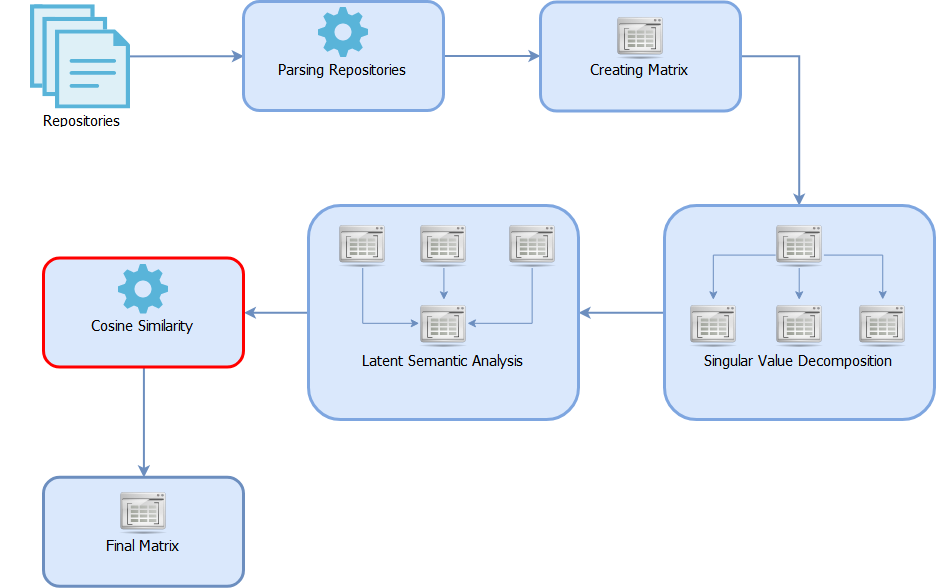
\includegraphics[width=0.8\textwidth]{images/Architecture5.png}
	\caption{Cosine Smilarity}
\end{figure}

As stated before, by cosine similarity we mean a measure of similarity between two non-zero vectors of an inner product space that measures the cosine of the angle between them, that is, how much they are close or far each other. As for the \emph{LSA} we re-implemented the operation from scratch, so the method take as input two vectors and computes the operation, such vectors are taken from the \emph{LSA} matrix, in such a way that every couple is taken into account. Since in the final matrix we will have the simlarity between \emph{repo1 - repo2} and \emph{repo2 - repo1}, we computed the cosine only in the upper triangular matrix to cut half of the calculation.

\begin{figure}[!h]
	\centering
	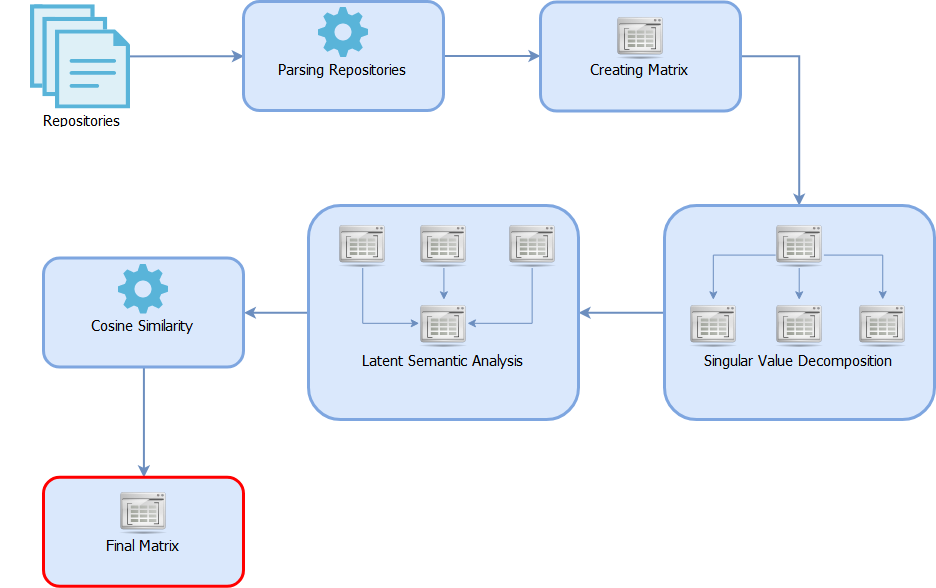
\includegraphics[width=0.8\textwidth]{images/Architecture6.png}
	\caption{Final Matrix}
\end{figure}

At this stage the matrix is complete with \emph{580 * 580} in dimension, and with values between \emph{0.0} and \emph{1.0}.
This matrix is actually a collection of vectors, representing the similarity of a project with all the other projects.
To be more formal the final matrix $\| M \|$ is square matrix whose rows and columun represents projects. In particular, for any two project $P_i$ and $P_j$, each element of the matrix $M_{i,j}$ represents the similarity score defined as follows: \\

\begin{equation}
  M_{i,j}=\begin{cases}
    0\leq M \leq 1 \; \; \; \text{if i} \neq \text{j}\\
    \\
    1 \; \; \; \text{if i = j}.
  \end{cases}
\end{equation}\\

There is one more step for \CLAN, since the approach consider the matrices separately, that is, at this stage we have two different matrices, one for the imports and one for the methods. So we have to sum up both in order to get the final one.

%%%%%%%%%%%%%%%%%%%%%%%%%%%%%%%%%%%%%%%%%%%%%%%%%%%%%%%%%%%%%%%%%%%%%%%%%%%%%%%%%%%%%%%%%%%
%\newpage

\section{Tools and Libraries}

Our implementations have been done using Eclipse IDE Oxygen .2, and the following libraries:

\begin{itemize}
\item \textbf{org.eclipse.jdt.core 3.10.0}. This is the core part of Eclipse's Java development tools. It contains the non-UI support for compiling and working with Java code, including the following:
	\begin{itemize}
	\item An incremental or batch Java compiler that can run standalone or as part of the Eclipse IDE.
	\item Java source and class file indexer and search infrastructure.
	\item A Java source code formatter.
	\item APIs for code assist, access to the AST and structured manipulation of Java source.
	\end{itemize}
\item \textbf{eclipse-astparser 8.1}: This is used to analyze the AST at runtime on Eclipse.
\item \textbf{commons-math3 3.6.1}: Commons Math is a library of lightweight, self-contained mathematics and statistics components addressing the most common problems not available in the Java programming language or Commons Lang. 
In particular used to compute the SVD, singular value decomposition.
\item \textbf{commons-text 1.2}: Apache Commons Text is a library focused on algorithms working on strings. 
\item \textbf{javaparser-core 3.5.14}: This is a library for parsing the java files.
\item \textbf{ejml-0.33}: Efficient Java Matrix Library (EJML) is a linear algebra library for manipulating real/complex/dense/sparse matrices. Its design goals are; 1) to be as computationally and memory efficient as possible for both small and large matrices, and 2) to be accessible to both novices and experts.These goals are accomplished by dynamically selecting the best algorithms to use at runtime, clean API, and multiple interfaces.
\end{itemize}

%%%%%%%%%%%%%%%%%%%%%%%%%%%%%%%%%%%%%%%%%%%%%%%%%%%%%%%%%%  
	\clearpage
	%	
	\chapter{Evaluation}
	\label{sec:Evaluation}
	%\section{Overview}
%As stated before we opted for \emph{MUDABLUE} and \emph{CLAN}. The rationale behind the selection of these approaches is that they are well-established algorithms. 





In this section we discuss the process that has been conceived and applied to evaluate the performance the four approaches introduced in Chapter~\ref{sec:Implementation}. To this end, the evaluation process that has been applied is shown in Figure~\ref{fig:EvaluationProcess} and consists of activities and artifacts that are going to be explained later on this chapter. In particular, a set of Java projects (Section~\ref{sec:Dataset}) has been crawled to feed as input for the computation by all approaches, \ie \MUDABlue, \CLAN, \RepoPal, and \CrossSim. Afterwards, a set of projects is selected as queries to compute similarities against all the remaining OSS projects (Section~\ref{sec:Queries}). Once the scores have been computed, for each similarity tool, some of the top similar projects are chosen, and mixed to be evaluated by humans (Section~\ref{sec:UserStudy}). The results are then evaluated using various quality metrics (Section~\ref{sec:Metrics}).


\begin{figure}[h!]
	\centering
	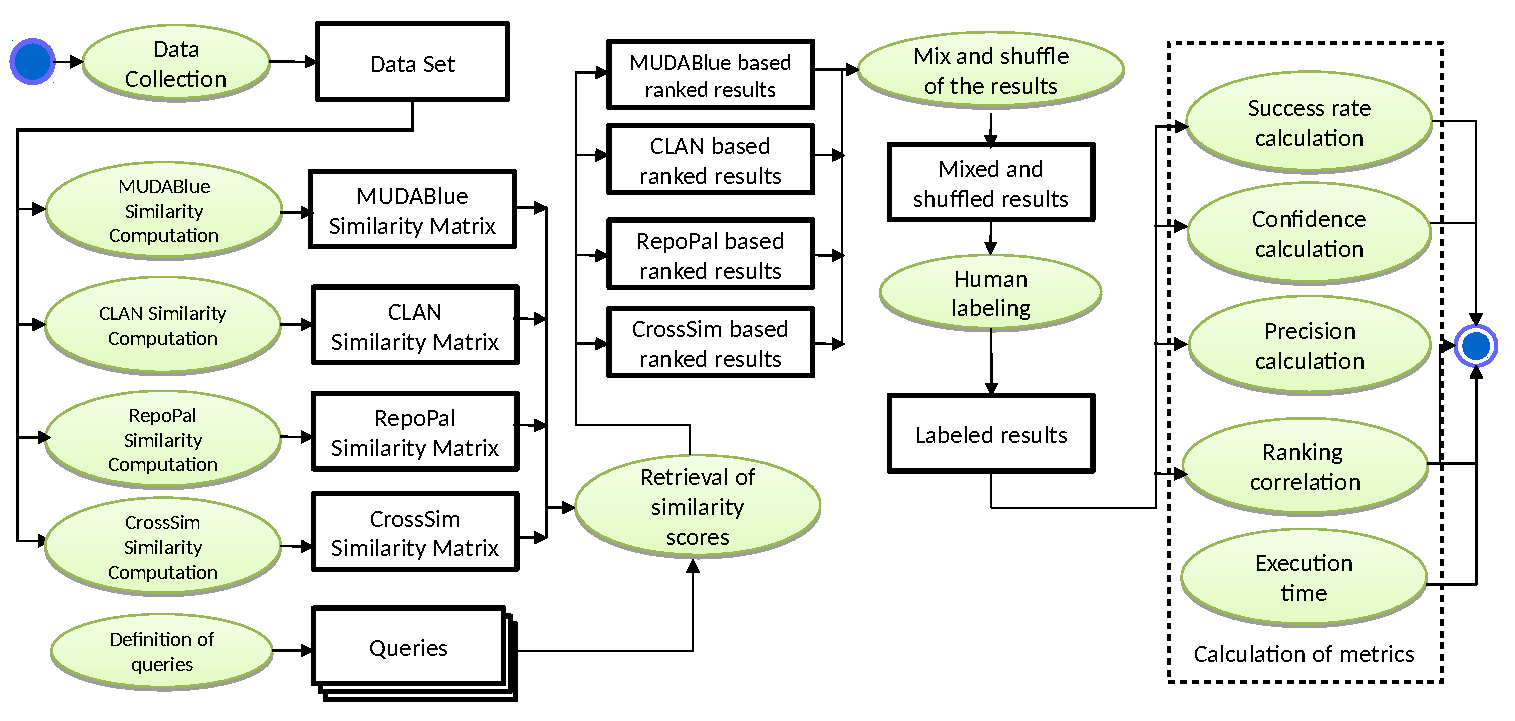
\includegraphics[width=0.99\linewidth]{images/EvaluationProcess}
	\caption{Evaluation process}
	\label{fig:EvaluationProcess}
\end{figure}








\section{Dataset} \label{sec:Dataset}

To serve as input for the evaluation, it is necessary to populate a dataset that meets the requirements by all four approaches. By MUDABlue and CLAN, there are no specific requirements since both metrics rely solely on source code to function. However, for CrossSim, we consider only projects that satisfy certain criteria. In particular, we collected projects that meet the following requirements:

\begin{itemize}
	\item Being GitHub Java projects; 
	\item Providing the specification of their dependencies by means of \code{code.xml} or \code{gradle} files;
	\item Including at least $9$ dependencies. A project with no or little information about dependencies may adversely affect the performance of \CrossSim; 
	\item Having the \code{README.md} file available.
\end{itemize}

Furthermore, we realized that the final outcomes of a similarity algorithm are to be validated by human beings, and in case the projects are irrelevant by their very nature, the perception given by human evaluators would also be \emph{dissimilar} in the end. This is valueless for the evaluation of similarity. Thus, to facilitate the analysis, instead of crawling projects in a random manner, we first observed projects in some specific categories (e.g. PDF processors, JSON parsers, Object Relational Mapping projects, and Spring MVC related tools). Once a certain number of projects for each category had been obtained, we also started collecting randomly to get projects from various categories.

Using the GitHub API\footnote{GitHub API: \url{https://developer.github.com/v3/}}, we crawled projects to provide input for the evaluation. Though the number of projects that fulfill the requirements of a single approach, i.e. either RepoPal or CrossSim, is high, the number of projects that meet the requirements of both approaches is considerably lower. For example, a project contains both \code{pom.xml} and \code{README.md}, albeit having only $5$ dependencies, does not meet the constraints and must be discarded. The crawling is time consuming as for each project, at least $6$ queries must be sent to get the relevant data. GitHub already sets a rate limit for an ordinary account\footnote{GitHub Rate Limit: \url{https://developer.github.com/v3/rate_limit/}}, with a total number of $5,000$ API calls per hour being allowed. And for the search operation, the rate is limited to $30$ queries per minute. Due to these reasons, we ended up getting a dataset of $580$ projects that are eligible for the evaluation. The dataset we collected and the CrossSim tool are already published online for public usage \cite{CROSSSIM-DATA}.

%\subsection{Data collection} \label{sec:DataCollection}
%In addition, to facilitate the evaluation of similarity and clustering techniques, instead of crawling projects in a random manner, we first observed projects in some specific categories. We suppose that the evaluation might lead to a cumbersome process if we consider arbitrary projects which are generally not related. The final outcomes of a similarity algorithm need to be validated by human beings, and given that the projects are irrelevant by their very nature, the perception given by human evaluators would also be \emph{dissimilar} in the end, and this is valueless for the evaluation of similarity. 

\begin{table}[h!]
%	\small
	\centering
	\begin{tabular}{|p{0.80cm}|p{6.00cm}|p{2.80cm}|}  \hline
		{\bf No.} & {\bf Name} & {\bf \# of Projects} \\  \hline
		1 & SPARQL, RDF, Jena Apache & 21 \\  \hline
		2 & PDF Processor & 8  \\  \hline
		3 & Selenium Web Test & 26  \\  \hline
		4 & ORM & 13  \\  \hline
		5 & Spring MVC & 51  \\  \hline
		6 & Music Player & 25  \\  \hline
		7 & Boilerplate & 38  \\  \hline
		8 & Elastic Search & 55  \\  \hline
		9 & Hadoop, MapReduce & 52  \\  \hline
		10 & JSON & 20  \\  \hline
		11 & Miscellaneous Categories & 271  \\  \hline
	\end{tabular}
	\caption[List of software categories]{List of software categories}
	\label{tab:Categories}
\end{table}


Further than collecting projects for each category, we also started collecting random projects. These projects serve as a means to test the stability of the algorithms. If the algorithms work well, they will not perceive newly added random projects as similar to projects of some other specific categories. To this end, the categories and their corresponding cardinality to be studied in our evaluation are listed in Table \ref{tab:Categories}. This is an approximate classification since a project might belong to more than one category.

As can be seen in Table \ref{tab:Categories}, among $580$ considered projects, $309$ of them belong to some specific categories, such as \emph{SPARQL, RDF, Jena Apache}, \emph{Selenium Test}, \emph{Elastic Search}, \emph{Spring MVC}, etc. The other $271$ projects being selected randomly belong to \emph{Miscellaneous Categories}. These categories disperse in several domains and sometimes it happens that there is only one project in a category. For the sake of clarity, we do not introduce the list of the categories in this thesis.

%The random projects are used as a means to.
%From the dataset, a graph is built using the relationships in Section~\ref{sec:GraphRepresentation}. %There, nodes are either users, dependencies or projects and each is encoded using a unique number across the whole graph. Edges represent the corresponding relationships between users and projects or between dependencies and projects. 
%\paragraph{\textbf{Application of RepoPal and CrossSim}}
%\noindent\emph{\textbf{Application of RepoPal and CrossSim}}



\section{Query definition} \label{sec:Queries}

Among $580$ projects in the dataset, $50$ have been selected as queries and they are listed in Table \ref{tab:Queries}. To aim for variety, the queries have been chosen to cover different categories, e.g.: SPARQL and RDF, Selenium Test, Elastic Search, Spring MVC, Hadoop, Music Player.

\begin{table}[!h]
	\footnotesize
	\centering
	\begin{tabular}{|p{0.80cm}|p{6.0cm}|p{0.80cm}|p{6.0cm}|}  \hline
		{\bf No.} & {\bf Name} & {\bf No.} & {\bf Name} \\  \hline
		1 & \href{https://github.com/neo4j-contrib/sparql-plugin}{neo4j-contrib/sparql-plugin}  & 26 & \href{https://github.com/mariamhakobyan/elasticsearch-river-kafka}{mariamhakobyan/elasticsearch-river-kafka} \\ \hline
		2 & \href{https://github.com/AskNowQA/AutoSPARQL}{AskNowQA/AutoSPARQL} & 27 & \href{https://github.com/OpenTSDB/opentsdb-elasticsearch}{OpenTSDB/opentsdb-elasticsearch} \\ \hline
		3 & \href{https://github.com/AKSW/Sparqlify}{AKSW/Sparqlify} & 28 & \href{https://github.com/codelibs/elasticsearch-cluster-runner}{codelibs/elasticsearch-cluster-runner} \\ \hline
		4 & \href{https://github.com/AKSW/SPARQL2NL}{AKSW/SPARQL2NL} & 29 & \href{https://github.com/opendatasoft/elasticsearch-plugin-geoshape}{opendatasoft/elasticsearch-plugin-geoshape} \\ \hline 
		5 & \href{https://github.com/pyvandenbussche/sparqles}{pyvandenbussche/sparqles} & 30 &  \href{https://github.com/huangchen007/elasticsearch-rest-command}{huangchen007/elasticsearch-rest-command} \\ \hline
		6 & \href{https://github.com/sayems/java.webdriver}{sayems/java.webdriver} & 31 & \href{https://github.com/pitchpoint-solutions/sfs}{pitchpoint-solutions/sfs} \\ \hline
		7 & \href{https://github.com/xebia/Xebium}{xebia/Xebium} & 32 & \href{https://github.com/javanna/elasticsearch-river-solr}{javanna/elasticsearch-river-solr} \\ \hline
		8 & \href{https://github.com/webdriverextensions/webdriverextensions}{webdriverextensions/webdriverextensions} & 33 & \href{https://github.com/mesos/hadoop}{mesos/hadoop} \\ \hline
		9 & \href{https://github.com/testIT-WebTester/webtester-core}{testIT-WebTester/webtester-core} & 34 & \href{https://github.com/pentaho/big-data-plugin}{pentaho/big-data-plugin} \\ \hline
		10 & \href{https://github.com/seleniumQuery/seleniumQuery}{seleniumQuery/seleniumQuery} & 35 & \href{https://github.com/asakusafw/asakusafw}{asakusafw/asakusafw} \\ \hline
		11 & \href{https://github.com/bonigarcia/webdrivermanager}{bonigarcia/webdrivermanager} & 36 & \href{https://github.com/klarna/HiveRunner}{klarna/HiveRunner} \\ \hline
		12 & \href{https://github.com/selenium-cucumber/selenium-cucumber-java}{selenium-cucumber/selenium-cucumber-java} & 37 &
		\href{https://github.com/sonalgoyal/hiho}{sonalgoyal/hiho} \\ \hline
		13 & \href{https://github.com/conductor-framework/conductor}{conductor-framework/conductor} & 38 & \href{https://github.com/pranab/beymani}{pranab/beymani} \\ \hline
		14 & \href{https://github.com/caelum/vraptor}{caelum/vraptor} & 39 & \href{https://github.com/lintool/Ivory}{lintool/Ivory} \\ \hline 
		15 & \href{https://github.com/caelum/vraptor4}{caelum/vraptor4} & 40 & \href{https://github.com/GoogleCloudPlatform/bigdata-interop}{GoogleCloudPlatform/bigdata-interop} \\ \hline
		16 & \href{https://github.com/KEN-LJQ/WMS}{KEN-LJQ/WMS} & 41 & \href{https://github.com/Conductor/kangaroo}{Conductor/kangaroo} \\ \hline
		17 & \href{https://github.com/white-cat/jeeweb}{white-cat/jeeweb} & 42 & \href{https://github.com/datasalt/pangool}{datasalt/pangool} \\ \hline
		18 & \href{https://github.com/livrospringmvc/lojacasadocodigo}{livrospringmvc/lojacasadocodigo} & 43 & \href{https://github.com/laserson/avro2parquet}{laserson/avro2parquet} \\ \hline
		19 & \href{https://github.com/spring-projects/spring-mvc-showcase}{spring-projects/spring-mvc-showcase} & 44 & \href{https://github.com/Knewton/KassandraMRHelper}{Knewton/KassandraMRHelper} \\ \hline
		20 & \href{https://github.com/sonian/elasticsearch-jetty}{sonian/elasticsearch-jetty} & 45 & \href{https://github.com/blackberry/KaBoom}{blackberry/KaBoom} \\ \hline
		21 & \href{https://github.com/dadoonet/spring-elasticsearch}{dadoonet/spring-elasticsearch} & 46 & \href{https://github.com/jt6211/hadoop-dns-mining}{jt6211/hadoop-dns-mining} \\ \hline
		22 & \href{https://github.com/elastic/elasticsearch-metrics-reporter-java}{elastic/elasticsearch-metrics-reporter-java} & 47 & \href{https://github.com/psaravan/JamsMusicPlayer}{psaravan/JamsMusicPlayer} \\ \hline
		23 & \href{https://github.com/elastic/elasticsearch-support-diagnostics}{elastic/elasticsearch-support-diagnostics} & 48 & \href{https://github.com/TheAndroidMaster/Pasta-Music}{TheAndroidMaster/Pasta-Music} \\ \hline
		24 & \href{https://github.com/SpringDataElasticsearchDevs/spring-data-elasticsearch}{SpringDataElasticsearchDevs/spring-data-elasticsearch} & 49 & \href{https://github.com/SubstanceMobile/GEM}{SubstanceMobile/GEM} \\ \hline
		25 & \href{https://github.com/javanna/elasticshell}{javanna/elasticshell} & 50 & \href{https://github.com/markzhai/LyricHere}{markzhai/LyricHere} \\ \hline
		
	\end{tabular}
	\caption[List of queries]{List of queries for evaluation}
	\label{tab:Queries}
\end{table}


% Three postgraduate students participated in the user study with two of them being
% Given a query, a user study is performed Evaluators are asked to label the similarity for each pair of projects (i.e., $<$\textit{query, retrieved project}$>$) with regards to their application domains and functionalities using the scales listed in Table \ref{tab:Scales}. 

%\section{Retrieval of similarity scores}
%
%Our evaluation has been conducted in line with some other existing studies \cite{Lo:2012:DSA:2473496.2473616},\cite{McMillan:2012:DSS:2337223.2337267},\cite{10.1109/SANER.2017.7884605}. For each query, similarity is computed against all the remaining projects in the dataset using \CrossSim. From the retrieved projects, only top $5$ are selected for evaluation. For each query, similarity is also computed using $RepoPal$ and other similarity metrics in Section \ref{sec:Baselines} to get the top-$5$ most similar retrieved projects.
%


\section{User Study} \label{sec:UserStudy}

%We involved a group of $15$ people software developers who have at least 5 years of experience in the user study. To get information about the participants related to their programming experience, we sent them a questionnaire similar to the one presented in \cite{McMillan:2012:DSS:2337223.2337267}. According to the survey, we found out that most developers use StackOverflow to search for code. %\footnote{\url{http://www.cs.wm.edu/semeru/clan/CaseStudyMaterials.zip}}. 
%Three postgraduate students in Computer Science who possess a good programming experience were invited to 
%In order to have a fair evaluation, for each query we mix and shuffle the top-$5$ results generated from the computation by all similarity metrics in a single file and present them to the evaluators. This mimics a \emph{taste test}\footnote{Taste Test: Is Bottled Better? \url{http://www.scwa.ca.gov/files/docs/outreach/water-ed/activities/Taste\%20Test.pdf}} where users are asked to evaluate a product, e.g. food or drink, without having a priori knowledge about what is being addressed. This helps eliminate any bias or prejudice against a specific similarity metric. Bias can be any preference given to a pre-known metric and any type of bias would considerably undermine the evaluation outcomes.%deteriorate
%In particular, given a query, a developer is asked to evaluate the similarity between the query and the corresponding retrieved projects. 


We performed a user study following the descriptions in \cite{Lo:2012:DSA:2473496.2473616},\cite{McMillan:2012:DSS:2337223.2337267},\cite{10.1109/SANER.2017.7884605} to evaluate the similarity between query projects and their corresponding retrieved projects. A group of $15$ software developers who have at least 5 years of experience took part in the experiments. In order to have a fair evaluation, for each query we mixed and shuffled the top-$5$ results generated from the computation by all similarity metrics in a single file and present them to the evaluators. This mimics a \emph{taste test} where users are asked to evaluate a product, \eg food or drink, without having a priori knowledge about what is being addressed \cite{Ghose2001},\cite{doi:10.1108/13522750810879048}. This aims at eliminating any bias or prejudice against a specific similarity metric. The participants are asked to label the similarity for each pair of projects (\ie $<$\textit{query, retrieved project}$>$) with regards to their application domains and functionalities using the scales listed in Table \ref{tab:Scales} \cite{McMillan:2012:DSS:2337223.2337267}. For example, an OSS project $p_{1}$ that performs the sending of files across a TCP/IP network is somehow similar to an OSS project $p_{2}$ that exchanges text messages between two users, \ie $Score(p_{1},p_{2})=3$. However an OSS project $p_{3}$ with the functionalities of a pure text editor is dissimilar to both $p_{1}$ and $p_{2}$, \ie $Score(p_{1},p_{2})=Score(p_{1},p_{3})=1$. Given a query, a retrieved project is considered as a \emph{false positive} if its similarity to the query is labeled as \code{Dissimilar} ($1$) or \code{Neutral} ($2$). In contrast, \emph{true positives} are those retrieved projects that have a score of $3$ or $4$, \ie \code{Similar} of \code{Highly similar}. A good similarity metric should produce as much true positives as possible.

\begin{table*}[h!]
	\centering
	\begin{tabular}{|p{3.0cm}|p{8.0cm}|p{1.0cm}|}  \hline
		{\bf Scale} & {\bf Description} & {\bf Score} \\  \hline
		Dissimilar & The functionalities of the retrieved project are completely different from those of the query project & 1 \\ \hline
		Neutral & The query and the retrieved projects share a few functionalities in common & 2 \\ \hline
		Similar & The two projects share a large number of tasks and functionalities in common & 3 \\ \hline
		Highly similar & The two projects share many tasks and functionalities in common and can be considered the same & 4 \\ \hline
	\end{tabular}
	\caption[The similarity scales]{Similarity scales}
	\label{tab:Scales}
\end{table*}


The participants are asked to label the similarity for each pair of projects (i.e., $<$\textit{query, retrieved project}$>$) with regards to their application domains and functionalities using the scales listed in Table \ref{tab:Scales}. For example, an OSS project $p_{1}$ that performs the sending of files across a TCP/IP network is somehow similar to an OSS project $p_{2}$ that exchanges text messages between two users, i.e. $Score(p_{1},p_{2})=3$. However an OSS project $p_{3}$ with the functionalities of a pure text editor is dissimilar to both $p_{1}$ and $p_{2}$, i.e. $Score(p_{1},p_{2})=Score(p_{1},p_{3})=1$. Given a query, a retrieved project is considered as a \emph{false positive} if its similarity to the query is labelled as Dissimilar ($1$) or Neutral ($2$). In contrast, \emph{true positives} are those retrieved projects that have a score of $3$ or $4$, i.e. Similar of Highly similar. A good similarity metric should produce as much true positives as possible.


\section{Evaluation Metrics} \label{sec:Metrics}

To evaluate the outcomes of the algorithms with respect to the user study, the following metrics have been considered as typically done in related work \cite{Lo:2012:DSA:2473496.2473616,McMillan:2012:DSS:2337223.2337267,10.1109/SANER.2017.7884605}:

\begin{itemize}
	\item \textit{Success rate}: if at least one of the top-5 retrieved projects is labelled \emph{Similar} or \emph{Highly similar}, the query is considered to be successful. {\em Success rate} is the ratio of successful queries to the total number of queries;
	\item \textit{Confidence}: Given a pair of $<$\textit{query, retrieved project}$>$ the confidence of an evaluator is the score she assigns to the similarity between the projects;
	\item \textit{Precision}: The precision for each query is the proportion of projects in the top-5 list that are labelled as \emph{Similar} or \emph{Highly similar} by humans. 
\end{itemize}

Further than the previous metrics, we introduce an additional one to measure the ranking produced by the similarity tools. For a query, a similarity tool is deemed to be good if all top-5 retrieved projects are relevant. In case there are false positives, i.e. those that are labeled \emph{Dissimilar} and \emph{Neutral}, it is expected that these will be ranked lower than the true positives. In case an irrelevant project has a higher rank than that of a relevant project, we suppose that the similarity tool is generating an improper recommendation. The \emph{Ranking} metric presented below is a means to evaluate whether a similarity metric produces properly ranked recommendations. 





\section{Results} \label{sec:Results}

To study the performance of the metrics in detecting similar projects for the set of queries, the following research questions are considered:

\newcommand{\rqfirst}{RQ$_1$: Which similarity metric yields a better performance in terms of Success rate, and Precision?}\textit{\textbf{\rqfirst}} 

By this question, we study the performance of different approaches.

\begin{figure}[!h]
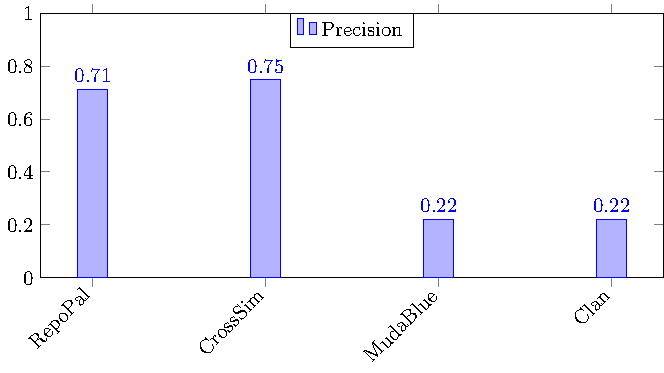
\includegraphics[width=10cm,height=15cm,keepaspectratio]{images/Precision.pdf}
\centering
\caption{Precision Comparison}
\label{fig:PrecisionC}
\end{figure}

Experimental results suggests that CrossSim approach overperforms all the other approaches, in particular Clan and MudaBlue.
Repopal got a good score, this means that is still a valid choice for similarity in the OSS environment.
The precision,as the figure~\ref{fig:PrecisionC} depicts, shows that CrossSim and Repopal got a score \emph{greater than 70\%}.
Clan and MudaBlue instead, reported a very low score, \emph{about 20\%}, on 10 queries evaluted, just 2 got a score \emph{$\geq3$}.

\begin{figure}[!h]
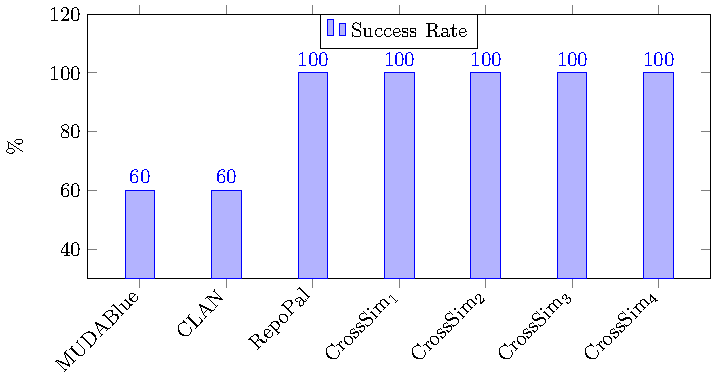
\includegraphics[width=10cm,height=15cm,keepaspectratio]{images/SuccessRate.pdf}
\centering
\caption{Success Rate Comparison}
\label{fig:SuccessC}
\end{figure}

Concerning the success rate, the results of CrossSim and Repopal are quite impressive, about \emph{100\%} of queries got score high, the situation is lower for Clan and MudaBlue that achieved just the \emph{60\%} of the queries. In order to calculate this values, we counted for each query how many votes were \emph{$\geq3$} divided then by 25, which is the number of queries.


\begin{figure}[!h]
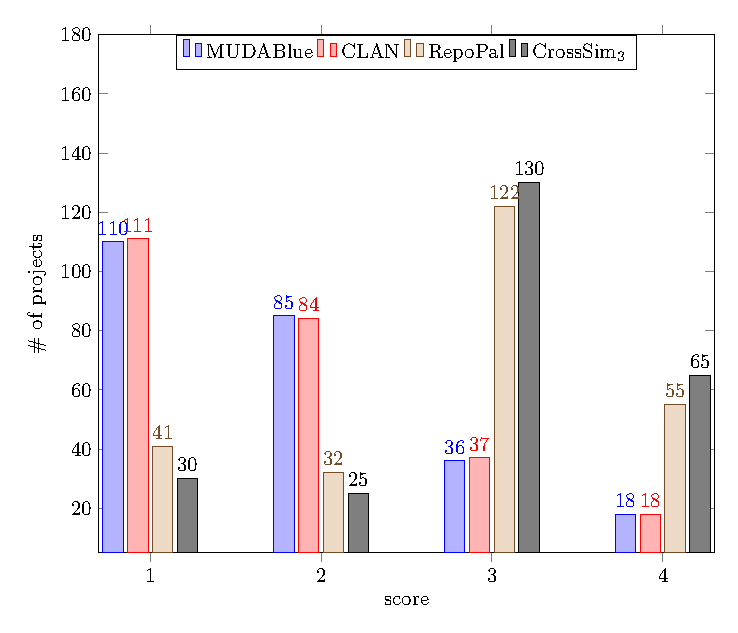
\includegraphics[width=10cm,height=15cm,keepaspectratio]{images/Confidence.pdf}
\centering
\caption{Confidence Comparison}
\label{fig:ConfidenceC}
\end{figure}

The confidence confirms what stated so far, the mojority of the votes for MudaBlue and Clan are between 1 and 2,that is, users evaluated as dissimilar most of the projects. For CrossSim the result is quite more nice, with 130 rank 3 votes and 60 rank 4 votes, so more than half results are good. Repopal also got a good evaluation, close to CrossSim but a bit lower.

\newcommand{\rqsecond}{RQ$_2$: Which similarity metric is more efficient?}\textit{\textbf{\rqsecond}} 

An important factor for a similarity metric is the ability to compute within an acceptable amount of time.

\begin{figure}[!h]
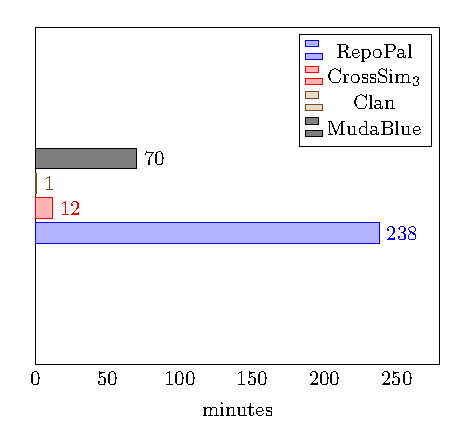
\includegraphics[width=8cm,height=13cm,keepaspectratio]{images/ExecutionTime.pdf}
\centering
\caption{Execution Time Comparison}
\label{fig:LabelC}
\end{figure}



\newcommand{\rqthird}{RQ$_3$: How does the graph structure affect the performance of \CrossSim?}\textit{\textbf{\rqthird}} 


When we consider \CrossSimA$_{1}$ in combination with \CrossSimA$_{2}$, the effect of the adoption of committers can be observed. \CrossSimA$_{1}$ gains a success rate of $100\%$, with a precision of $0.748$ and $63$ false positives. Whereas, the number of false positives by \CrossSimA$_{2}$ goes up to $76$, thereby worsening the overall performance considerably with $0.696$ being as the precision. The precision of \CrossSimA$_{2}$ is higher than those of $Readme$, $Dependency$, $Compound$, $Weighted$ $RepoPal$, but lower than those of $RepoPal$ and all of its \CrossSim counterparts. The performance degradation is further witnessed by considering \CrossSimA$_{3}$ and \CrossSimA$_{4}$ together. With respect to \CrossSimA$_{3}$, the number of false positives by \CrossSimA$_{4}$ increases by $5$ projects. We come to the conclusion that the inclusion of all developers who have committed updates at least once to a project in the graph is counterproductive as it adds a decline in precision. In this sense, we make an assumption that the deployment of a weighting scheme for developers may help counteract the degradation in performance. We consider the issue as our future work. 

Next, \CrossSimA$_{1}$ and \CrossSimA$_{3}$ are studied together to analyze the effect of the removal of the most frequent dependencies. \CrossSimA$_{3}$ outperforms \CrossSimA$_{1}$ as it gains a precision of $0.784$, the highest value among all, compared to $0.748$ by \CrossSimA$_{1}$. The removal of the most frequent dependencies helps also improve the performance of \CrossSimA$_{4}$ in comparison to \CrossSimA$_{2}$, which is a similar configuration, except that all dependencies are taken into account. Together, this implies that the elimination of too popular dependencies in the original graph is a profitable amendment. This is understandable once we get a deeper insight into the design of SimRank as already presented in Section \ref{sec:SimRank} and Figure \ref{fig:SimRank}. There, two projects are deemed to be similar if they share a same dependency, or in other words their corresponding nodes in the graph are pointed by a common node. However, with frequent dependencies as in Table \ref{tab:FrequentDeps} this characteristic may not hold anymore. Take as an example, two projects are pointed by a frequent dependency, e.g. \href{https://mvnrepository.com/artifact/junit/junit}{junit:junit} because they use JUnit\footnote{JUnit: Testing Framework for Java 8: \url{http://junit.org/junit5/}} for testing. And since testing is a common functionality of many software projects, it does not help contribute towards the characterization of a project and as a result, needs to be removed from similarity computation. 





\section{Threats to Validity}\label{sec:threatsValidity}

In this section, we investigate the threats that may affect the validity of the experiments as well as how we have tried to minimize them. In particular, we focus on the following threats to validity as discussed below. %internal and external 

\textit{\textbf{Internal validity}}  concerns any confounding factor that could influence our results.  We attempted to avoid any bias in the evaluation and assessment
phases: (\emph{i}) by involving three participants in the user study. In particular, the labeling results by one user were then double-checked by other two users to make sure that the outcomes were sound; (\emph{ii}) by completely automating the evaluation of the defined metrics without any manual intervention. Indeed, the implemented tools could be defective. To contrast and mitigate this threat, we have run several manual assessments and counter-checks.

\textit{\textbf{External validity}}  refers to the generalizability of obtained results and findings. Concerning the generalizability of our approach, we were able to consider a dataset of $580$ projects, due to the fact that the number of projects that meet the requirements of both RepoPal and CrossSim is low and thus required a prolonged crawling. During the data collection, we crawled both projects in some specific categories as well as random projects. The random projects served as a means to test the generalizability of our algorithm. If the algorithm works well, it will not perceive newly added random projects as similar to projects of the specific categories.

\textit{\textbf{Reliable validity}}  is related to the reproducibility of our experiments. To allow anyone to seamlessly replicate the evaluation, we made available the source code implementation of MUDABlue, CLAN, RepoPal, and CrossSim as also the dataset exploited in the paper in our GitHub repository \cite{CROSSSIM-DATA}.
	\clearpage
	%	
	\chapter{Conclusions}
	\label{sec:Conclusions}
	
Measuring similarities between software systems has been considered as a daunting task. Furthermore, considering the miscellaneousness of artifacts in open source software repositories, similarity computation becomes more complicated as many artifacts and several cross relationships prevail. Thus, choosing the right tool to compute software similarity is a question that may arise at any time. The current thesis attempts to address one of the issues in software similarity computation by performing a comprehensive evaluation on various techniques. We performed a literature review on different approaches for computing software similarity. We see that depending on the set of mined features, there are two main types of software similarity computation techniques. The first type is \textit{Low-level Similarity} where only low-level data, e.g., source code, byte code, function calls, API reference, etc. is considered. The second type is \textit{High-level Similarity} and it detects the semantic similarity using metadata, such as: topic distribution, readme file, description, star events, etc. Source code is not taken into account.

Most low-level similarity algorithms attempt to represent source code (and API calls) in a term-document matrix and then apply SVD to reduce dimensionality. The similarity is then computed as the cosine similarity between feature vectors. Among others, \MUDABlue \cite{10.1109/APSEC.2004.69}, \CLAN \cite{McMillan:2012:DSS:2337223.2337267}, and CLANdroid \cite{10.1109ICPC.2016.7503721} belong to this category. \CLAN includes API calls for computing similarity, whereas, by \MUDABlue, every word appearing in source code files is integrated into the term-document matrix. This makes the difference in the performance of the two algorithms in a way that the similarity scores of \CLAN reflect better the perception of humans of similarity than those of \MUDABlue. In contrast, high-level similarity techniques do not consider source code for similarity computation. They characterize software by exploiting available features such as descriptions, user reviews, and \code{README.MD} file. The similarity is computed as the cosine similarity of the corresponding feature vectors. For computing similarity between mobile applications, other specific features such as images and permissions are also incorporated. 

We re-implement four software similarity tools and conduct an empirical evaluation using a dataset of $580$ GitHub Java projects collected from GitHub. The obtained results are promising: by considering \MUDABlue, \CLAN, and \RepoPal as baseline, we demonstrated that \CrossSim is considered as a good candidate for computing similarities among open source software projects. \CrossSim is an extensible and flexible approach to calculate the similarity of open source projects. It can deal with various types of input project information that is represented in a homogeneous manner by means of graphs. By means of the proposed graph representation, it is possible to transform the relationships among various artifacts, e.g. developers, API utilizations, source code, interactions, into a mathematically computable format. In this sense, \CrossSim is a versatile similarity tool as it can accept various input features regardless of their format. %As long as the inputs are integrated into the graph, the similarity between different artifacts can then be computed using the augmented graph. 

%One of the most hard issue faced was related to the physical memory required to compute the Latent Semantic Analysis, for \MUDABlue in particular we got something like $700,000$ terms. This means that the required memory, only to manage the matrix was about 3Gb, this excluding all the memory used for other data structures and for the parsing. That's why we put a bound for the Eclipse virtual memory up to 8Gb and worked in two phase. During the first phase we collected all the terms by parsing everything and then, after an IDE restart, computing the LSA.





%\begin{itemize}
%	\item Study and Analysis of the problem. In this phase we have analyzed the similarity problem discovering that is well known problem studied in order to find a solution to some very interesting problems such as: (plagiarism detection, information retrieval,text classification, document clustering, topic detection and so on).In order to validate our novel approach we eventually decided to study in detail and implement two similarity calculator approaches: MudaBlue and Clan.
%	\item Implementation. The implementation phase covered a lot of aspects. First of all was necessary analyzing the projects by parsing each \emph{.java} file and then summing up everything in a \emph{Term-Document matrix}. We applied then, the core of the apporaches, the \emph{Latent Semantic Analysis}, applying then the cosine similarity on the matrix we got the final matrix ready to be evaluated. The Ide was Eclipse and the language Java, with a lot of supporting library.
%	\item Results Validation. At this stage we started the evaluation phase which consisted in a user study. We asked to a group of 10 people with experencie in Java delepoment, to rate a pull of queries provided by us. The results confirmed that CrossSim is a more precise method to calculate similarity with rispect to Clan and MudaBlue.
%\end{itemize}

%%%%%Future Works%%%%%

%Since the evualation was succesfully, in the sense that, results confirmed that CrossSim is a valuable similarity approach, the idea is to continue the development of the other features that still are missing (e.g. Code snippet suggestion, Api reccomandation).

%In order to provide such a baseline was mandatory to find some similar approach, we decided to use MudaBlue and Clan which are two close approaches, since there weren't any implementation available we re-implemented them from scratch. The contribute can be summarized as follows:

%Measuring similarities between software systems has been considered as a daunting task \cite{Chen:2015:SFD:2684822.2685305},\cite{McMillan:2012:DSS:2337223.2337267}. Furthermore, considering the miscellaneousness of artifacts in open source software repositories, similarity computation becomes more complicated as many artifacts and several cross relationships prevail. Given the circumstances, choosing the right tool to compute software similarity is a question that may arise at any time. To this end, the current thesis attempts to address one of the issues in software similarity computation by performing a comprehensive evaluation on various techniques. In particular, we re-implement four software similarity tools and conduct an empirical evaluation using a dataset collected from GitHub.
	\clearpage
	


%----------------------------------------------------------------------------------------
%	THESIS CONTENT - APPENDICES
%----------------------------------------------------------------------------------------

\appendix % Cue to tell LaTeX that the following "chapters" are Appendices

% Include the appendices of the thesis as separate files from the Appendices folder
% Uncomment the lines as you write the Appendices

\include{src/AppendixA}

%----------------------------------------------------------------------------------------
%	BIBLIOGRAPHY
%----------------------------------------------------------------------------------------

\printbibliography[heading=bibintoc]

%----------------------------------------------------------------------------------------

\end{document}  
